\chapter{Projeto Preliminar}

\section{Definição do Perfil da Asa}

Inicialmente, foram identificados os perfis utilizados nas aeronaves de referência, conforme a Tabela \ref{tab:perfiscomparativos}. Os dados foram obtidos no \textit{The Incomplete Guide to Airfoil Usage} \cite{uiuc_airfoil_database}, exceto para o Xian MA600, para o qual foi utilizada a referência da Antonov Company sobre o An-24 \cite{antonov_an24}. Não foi encontrada uma fonte confiável para o perfil do Ilyushin Il-114-300.

\begin{table}[H]
\centering
\caption{Perfis aerodinâmicos das aeronaves analisadas.}
\label{tab:perfiscomparativos}
\begin{tabular}{|l|c|c|}
\hline
\textbf{Aeronave} & \textbf{Perfil na Raiz} & \textbf{Perfil na Ponta} \\ \hline
ATR-72 & NACA 43018 Modificado & NACA 43013 Modificado  \\ \hline
CASA C-295 & NACA 65-218 & NACA 65-218 \\ \hline
British Aerospace ATP & NACA 23018 & NACA 4412 \\ \hline
NAMC YS-11 & NACA 64A218 & NACA 64A412 \\ \hline
Xian MA600 & TsAGI S-5-18 & TsAGI S-3-13 \\ \hline
\end{tabular}
\end{table}

Entre as aeronaves analisadas, observa-se a utilização de perfis NACA de cinco dígitos em projetos de referência, como o ATR-72 e o British Aerospace ATP. Essa família foi adotada como ponto de partida para o presente projeto. Sua nomenclatura é definida por:

\begin{itemize}
    \item O primeiro dígito multiplicado por 0,15 define o coeficiente de sustentação de projeto. Para o NACA 43018, $C_l = 4 \cdot 0,15 = 0,60$;
    \item O segundo e o terceiro dígitos estão associados à posição de máxima curvatura. Para o NACA 43018, o número 30 corresponde a $15\%$ da corda;
    \item O terceiro dígito igual a 0 indica uma linha média convencional, não reflexa;
    \item Os dois últimos dígitos representam a espessura relativa máxima, resultando em $t/c=18\%$.
\end{itemize}

A seguir, estima-se o coeficiente de sustentação de projeto para a condição de cruzeiro.

\subsection{Análise de Condição de Cruzeiro}

Considerando cruzeiro a 20.000 ft, equivalente a 80\% do teto operacional, o coeficiente de sustentação é estimado por:

\begin{equation}
\label{eq:ClCruseiro}
    C_{l_{cruise}} = \frac{MTOW \cdot g}{\frac{1}{2}\rho_{cruise} V_{cruise}^2 S_{wing}} = 0,48
\end{equation}
Onde o $MTOW = 22680 \ kg$, $V_{cruise} = 260 \ kt$, $S = 74,1 \ m^2$.

Com o valor obtido pela Eq. \ref{eq:ClCruseiro}, podemos estimar o coeficiente que o perfil aerodinâmico deve gerar levando em conta efeitos tridimensionais e de perfil ideal, tal que Raymer \cite{raymer2018} indica:

\begin{equation}
\label{eq:Clperfildeverdade}
    C_l = C_{l_{cruise}}/0,86 = 0,56
\end{equation}

\subsection{Comparação de Eficiência Aerodinâmica}
\label{subsec:comparacao_ld_perfis}

Para $C_l \approx 0,56$, comparou-se o NACA 43018, utilizado como representante preliminar da família NACA 430XX, com os perfis laminares NACA 64-215 e NACA 65(2)-215. As polares foram obtidas no AirfoilTools \cite{airfoiltools} e a comparação de $C_l/C_d$ é apresentada na Figura \ref{fig:comparacao_clcd_cl}.

\begin{figure}[H]
    \centering
    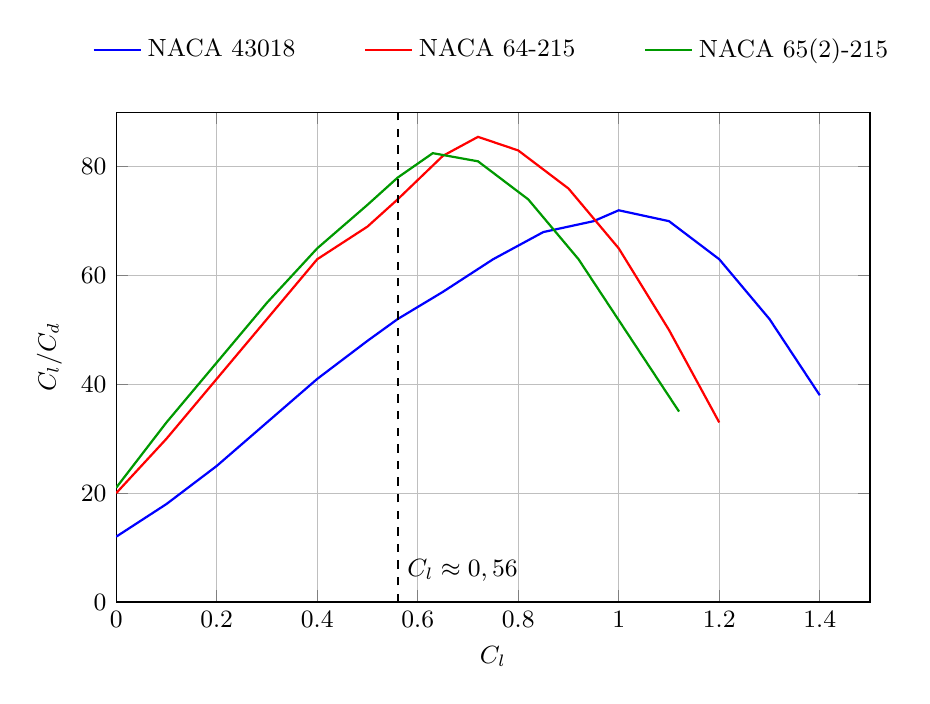
\begin{tikzpicture}
    \begin{axis}[
        width=0.92\linewidth,
        height=7.8cm,
        xlabel={$C_l$},
        ylabel={$C_l/C_d$},
        xmin=0, xmax=1.50,
        ymin=0, ymax=90,
        grid=major,
        tick label style={font=\small},
        label style={font=\small},
        every axis plot/.append style={thick},
        legend columns=3,
        legend style={
            at={(0.5,1.08)},
            anchor=south,
            font=\small,
            draw=none,
            fill=none,
            /tikz/every even column/.append style={column sep=0.8cm}
        }
    ]

    % NACA 43018
    \addplot[color=blue] coordinates {
        (0.00,12)
        (0.10,18)
        (0.20,25)
        (0.30,33)
        (0.40,41)
        (0.50,48)
        (0.56,52)
        (0.65,57)
        (0.75,63)
        (0.85,68)
        (0.95,70)
        (1.00,72)
        (1.10,70)
        (1.20,63)
        (1.30,52)
        (1.40,38)
    };
    \addlegendentry{NACA 43018}

    % NACA 64-215
    \addplot[color=red] coordinates {
        (0.00,20)
        (0.10,30)
        (0.20,41)
        (0.30,52)
        (0.40,63)
        (0.50,69)
        (0.56,74)
        (0.65,82)
        (0.72,85.5)
        (0.80,83)
        (0.90,76)
        (1.00,65)
        (1.10,50)
        (1.20,33)
    };
    \addlegendentry{NACA 64-215}

    % NACA 65(2)-215
    \addplot[color=green!60!black] coordinates {
        (0.00,21)
        (0.10,33)
        (0.20,44)
        (0.30,55)
        (0.40,65)
        (0.50,73)
        (0.56,78)
        (0.63,82.5)
        (0.72,81)
        (0.82,74)
        (0.92,63)
        (1.02,49)
        (1.12,35)
    };
    \addlegendentry{NACA 65(2)-215}

    % Condição de projeto
    \addplot[color=black, dashed] coordinates {(0.56,0) (0.56,90)};
    \node[anchor=south west, font=\small]
        at (axis cs:0.56,2) {$C_l \approx 0,56$};

    \end{axis}
    \end{tikzpicture}

    \caption{Eficiência aerodinâmica dos perfis avaliados.}
    \label{fig:comparacao_clcd_cl}
\end{figure}

Os perfis laminares da série NACA 6 apresentaram maior eficiência aerodinâmica na condição analisada. Entretanto, sua vantagem depende da manutenção de uma superfície limpa e com baixa rugosidade, condição que pode ser comprometida por contaminação, chuva, insetos e formação de gelo. Por esse motivo, nesta etapa do projeto não foi adotado um perfil laminar como requisito, mantendo-se a família NACA 430XX como referência por apresentar maior robustez operacional.

Também é prevista a utilização de um sistema de proteção contra gelo nos bordos de ataque da asa e das empenagens, com a solução de degelo ou antigelo a ser definida em etapas posteriores do projeto. Essa previsão deve ser considerada na geometria e no acabamento superficial do bordo de ataque, especialmente por sua influência sobre a transição da camada limite e, consequentemente, sobre os benefícios associados ao escoamento laminar.

Definida a família do perfil, a seção seguinte determina a espessura relativa necessária ao longo da semi-envergadura a partir dos requisitos estruturais da asa.


\subsection{Análise da Espessura Relativa} 
\label{analise_espessura}

Para estimar os esforços na asa, adotou-se o método de Stender, no qual a sustentação local é proporcional a uma corda equivalente dada pela média geométrica entre as cordas trapezoidal e elíptica.

Utilizando as dimensões de asa previamente definidas: $b = 28,5$ m, $\lambda = 0,405$, AR = 10,96 e $S = 74,1$ $m^2$; e considerando a condição crítica de MTOW com um fator de carga igual a 2,5, a distribuição de sustentação ao longo da semi-envergadura da asa da aeronave é apresentada na Figura \ref{fig:distribuição de sustentação}.

\begin{figure} [H]
    \centering
    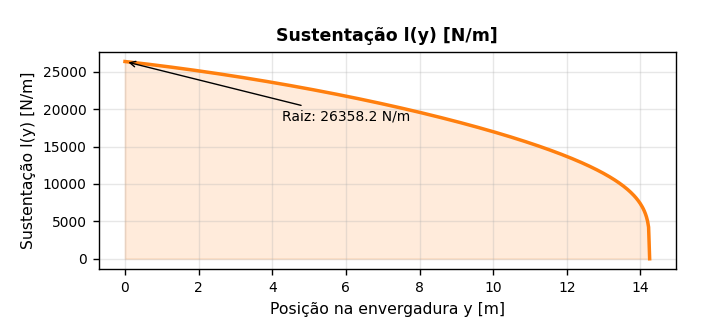
\includegraphics[width=0.7\linewidth]{images/Distribuição de Sustentação.png}
    \caption{Distribuição de sustentação ao longo da semi-envergadura.}
    \label{fig:distribuição de sustentação}
\end{figure}

Vale pontuar que, para a obtenção dessa distribuição por meio do método de Stender, foi feita uma discretização da semi-asa em 500 pontos. 

A partir da distribuição de sustentação, a força cortante e o momento fletor foram obtidos por integração numérica pelo método do trapézio:

\begin{equation}
    V(y) = \int_{0}^{\frac{b}{2}} L(y) \, dy
    \label{cortante}
\end{equation}

\begin{equation}
    M(y) = \int_{0}^{\frac{b}{2}} V(y) \, dy
    \label{momento fletor}
\end{equation}

\begin{figure} [H]
    \centering
    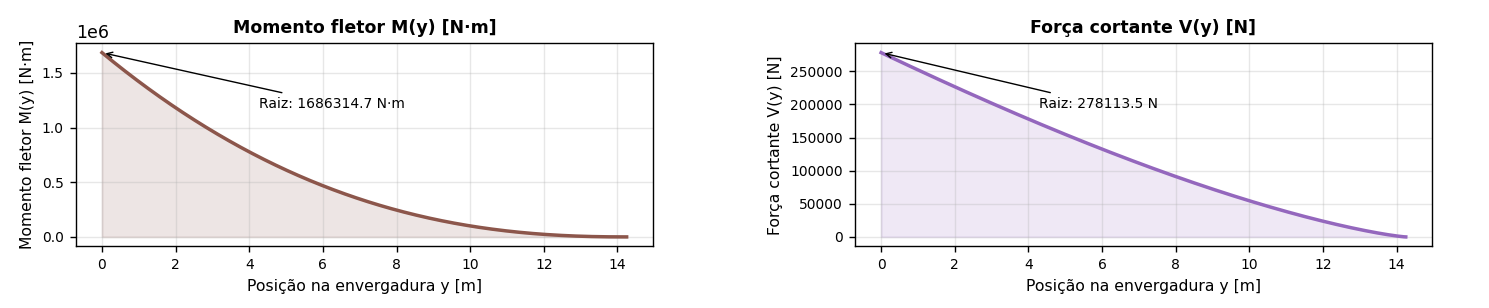
\includegraphics[width=1.0\linewidth]{images/Cortantes e Momentos na Asa.png}
    \caption{Momento fletor e força cortante ao longo da semi-envergadura.}
    \label{fig:Momentos e Cortantes na Asa}
\end{figure}

Para estimar a espessura mínima do perfil, considerou-se uma longarina equivalente de seção I, cuja altura $h$ é limitada pelos esforços locais. Foram adotadas mesas com espessura de $5\%h$ e largura de $25\%h$, e alma com espessura de $10\%h$. As tensões foram avaliadas no bordo da mesa, na junção mesa-alma e na linha neutra, por:

\begin{equation}
    \sigma=\frac{M \cdot z}{I}
    \label{tensão normal}
\end{equation}

\begin{equation}
    \tau = \frac{V \cdot Q}{I \cdot t}
    \label{tensão cisalhante}
\end{equation}

onde t é a espessura da chapa do ponto analisado.

A tensão equivalente de Von Mises foi comparada ao limite de escoamento do alumínio 7075-T6, adotado como $\sigma_y=480$ MPa:

\begin{equation}
    \sigma_{eq} = \sqrt{\sigma^2+3\tau^2}
    \label{tensão equivalente}
\end{equation}

Como a altura $h$ da longarina limita a espessura do perfil, adotou-se $t/c=h/c$ para avaliar a espessura relativa mínima ao longo da semi-envergadura. Foram analisados valores entre 9\% e 21\%, conforme a Figura \ref{fig:tensão de von mises}.

\begin{figure} [H]
    \centering
    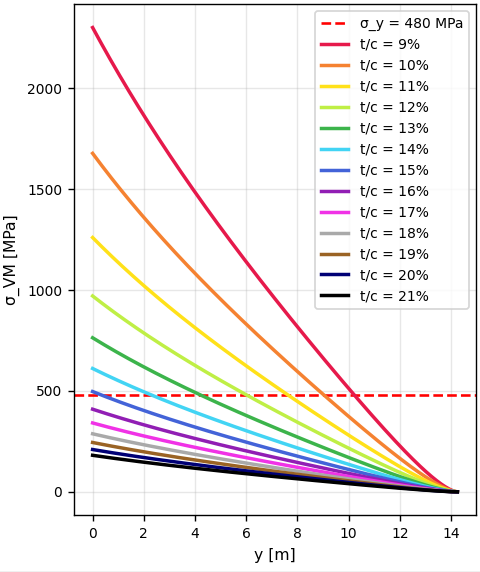
\includegraphics[width=0.5\linewidth]{images/Tensão de Von Mises.png}
    \caption{Tensão de Von Mises ao longo da semi-envergadura para diferentes espessuras relativas.}
    \label{fig:tensão de von mises}
\end{figure}

Na raiz, valores de $t/c \leq 15\%$ levam ao escoamento, enquanto na ponta todos os valores avaliados atendem ao critério estrutural. Visando reduzir o arrasto parasita, adotou-se o menor valor que atende ao critério em cada região: $t/c=16\%$ na raiz e $t/c=9\%$ na ponta, com transição linear entre ambos. A Figura \ref{fig:transição linear de perfil} confirma que a transição linear adotada permanece acima da espessura estrutural mínima ao longo de toda a semi-envergadura.

\begin{figure} [H]
    \centering
    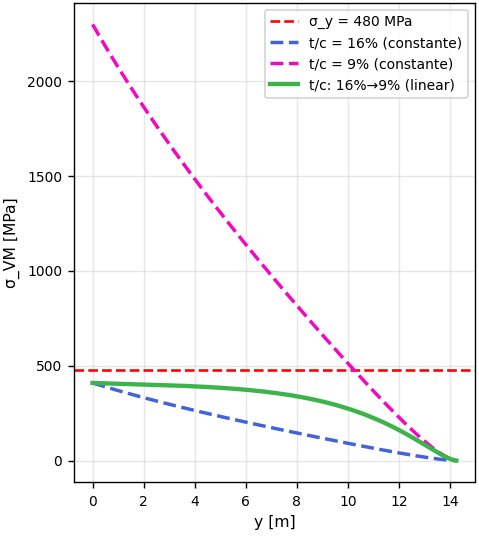
\includegraphics[width=0.5\linewidth]{images/Transição linear do perfil.png}
    \caption{Avaliação da transição linear dos perfis ao longo da semi-envergadura.}
    \label{fig:transição linear de perfil}
\end{figure}

\subsection{Definição Final do Perfil}
\label{subsec:definiçãoPerfil}

Portanto, reunindo todas as informações das últimas seções, os perfis definidos para a asa do projeto são:

\begin{itemize}
    \item Raiz da Asa: NACA 43016
    \item Ponta da Asa: NACA 43009
\end{itemize}

Eles são mostrados sobrepostos na Figura \ref{fig:PerfisDaAsa}.

\begin{figure} [H]
    \centering
    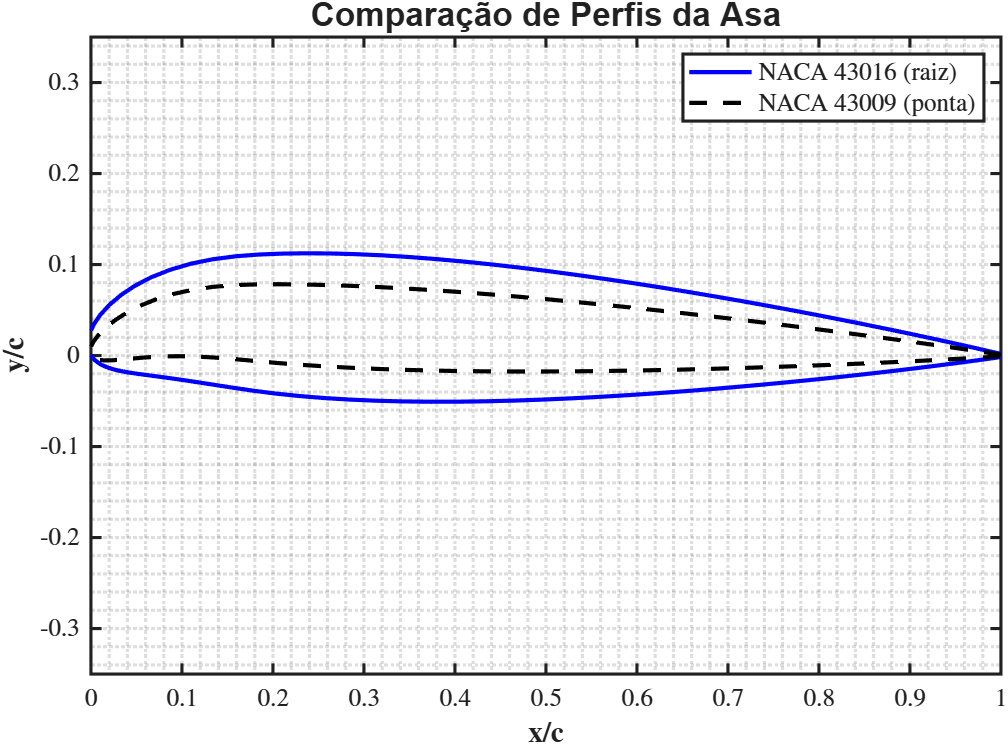
\includegraphics[width=0.6\linewidth]{images/PerfisDaAsa.png}
    \caption{Perfis da raiz e ponta de asa}
    \label{fig:PerfisDaAsa}
\end{figure}

\subsection{Análise Tridimensional da Asa no XFLR5}

A fim de verificar as curvas aerodinâmicas da asa, os valores da Tabela \ref{tab:dimensoes_conclusao} e os dados obtidos por análise no XFLR5 dos perfis obtidos na seção \ref{subsec:definiçãoPerfil} foram importados para a seção de desenho 3D no software mencionado.

\begin{figure}[H]
    \centering
    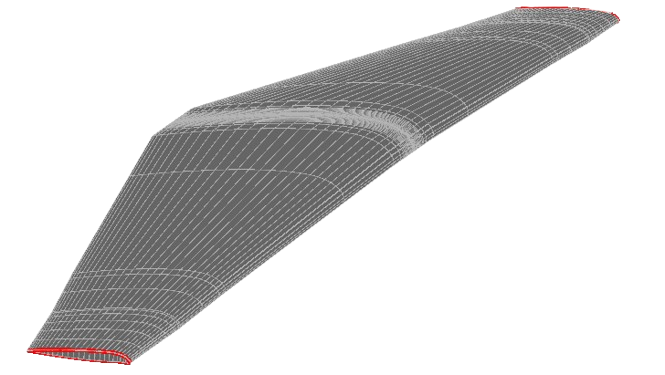
\includegraphics[width=0.8\linewidth]{images/AsaXFLR5.png}
    \caption{Asa desenhada no XFLR5}
    \label{fig:AsaXFLR5}
\end{figure}

Com isso, para a velocidade de cruzeiro $V_c = 260 \text{ kt} \approx 134 \text{ m/s}$, as seguintes curvas foram obtidas (Figuras \ref{fig:polar_arrasto} e \ref{fig:eficiencia_aero}):

\begin{figure}[H]
    \centering
    \begin{minipage}{0.48\textwidth}
        \centering
        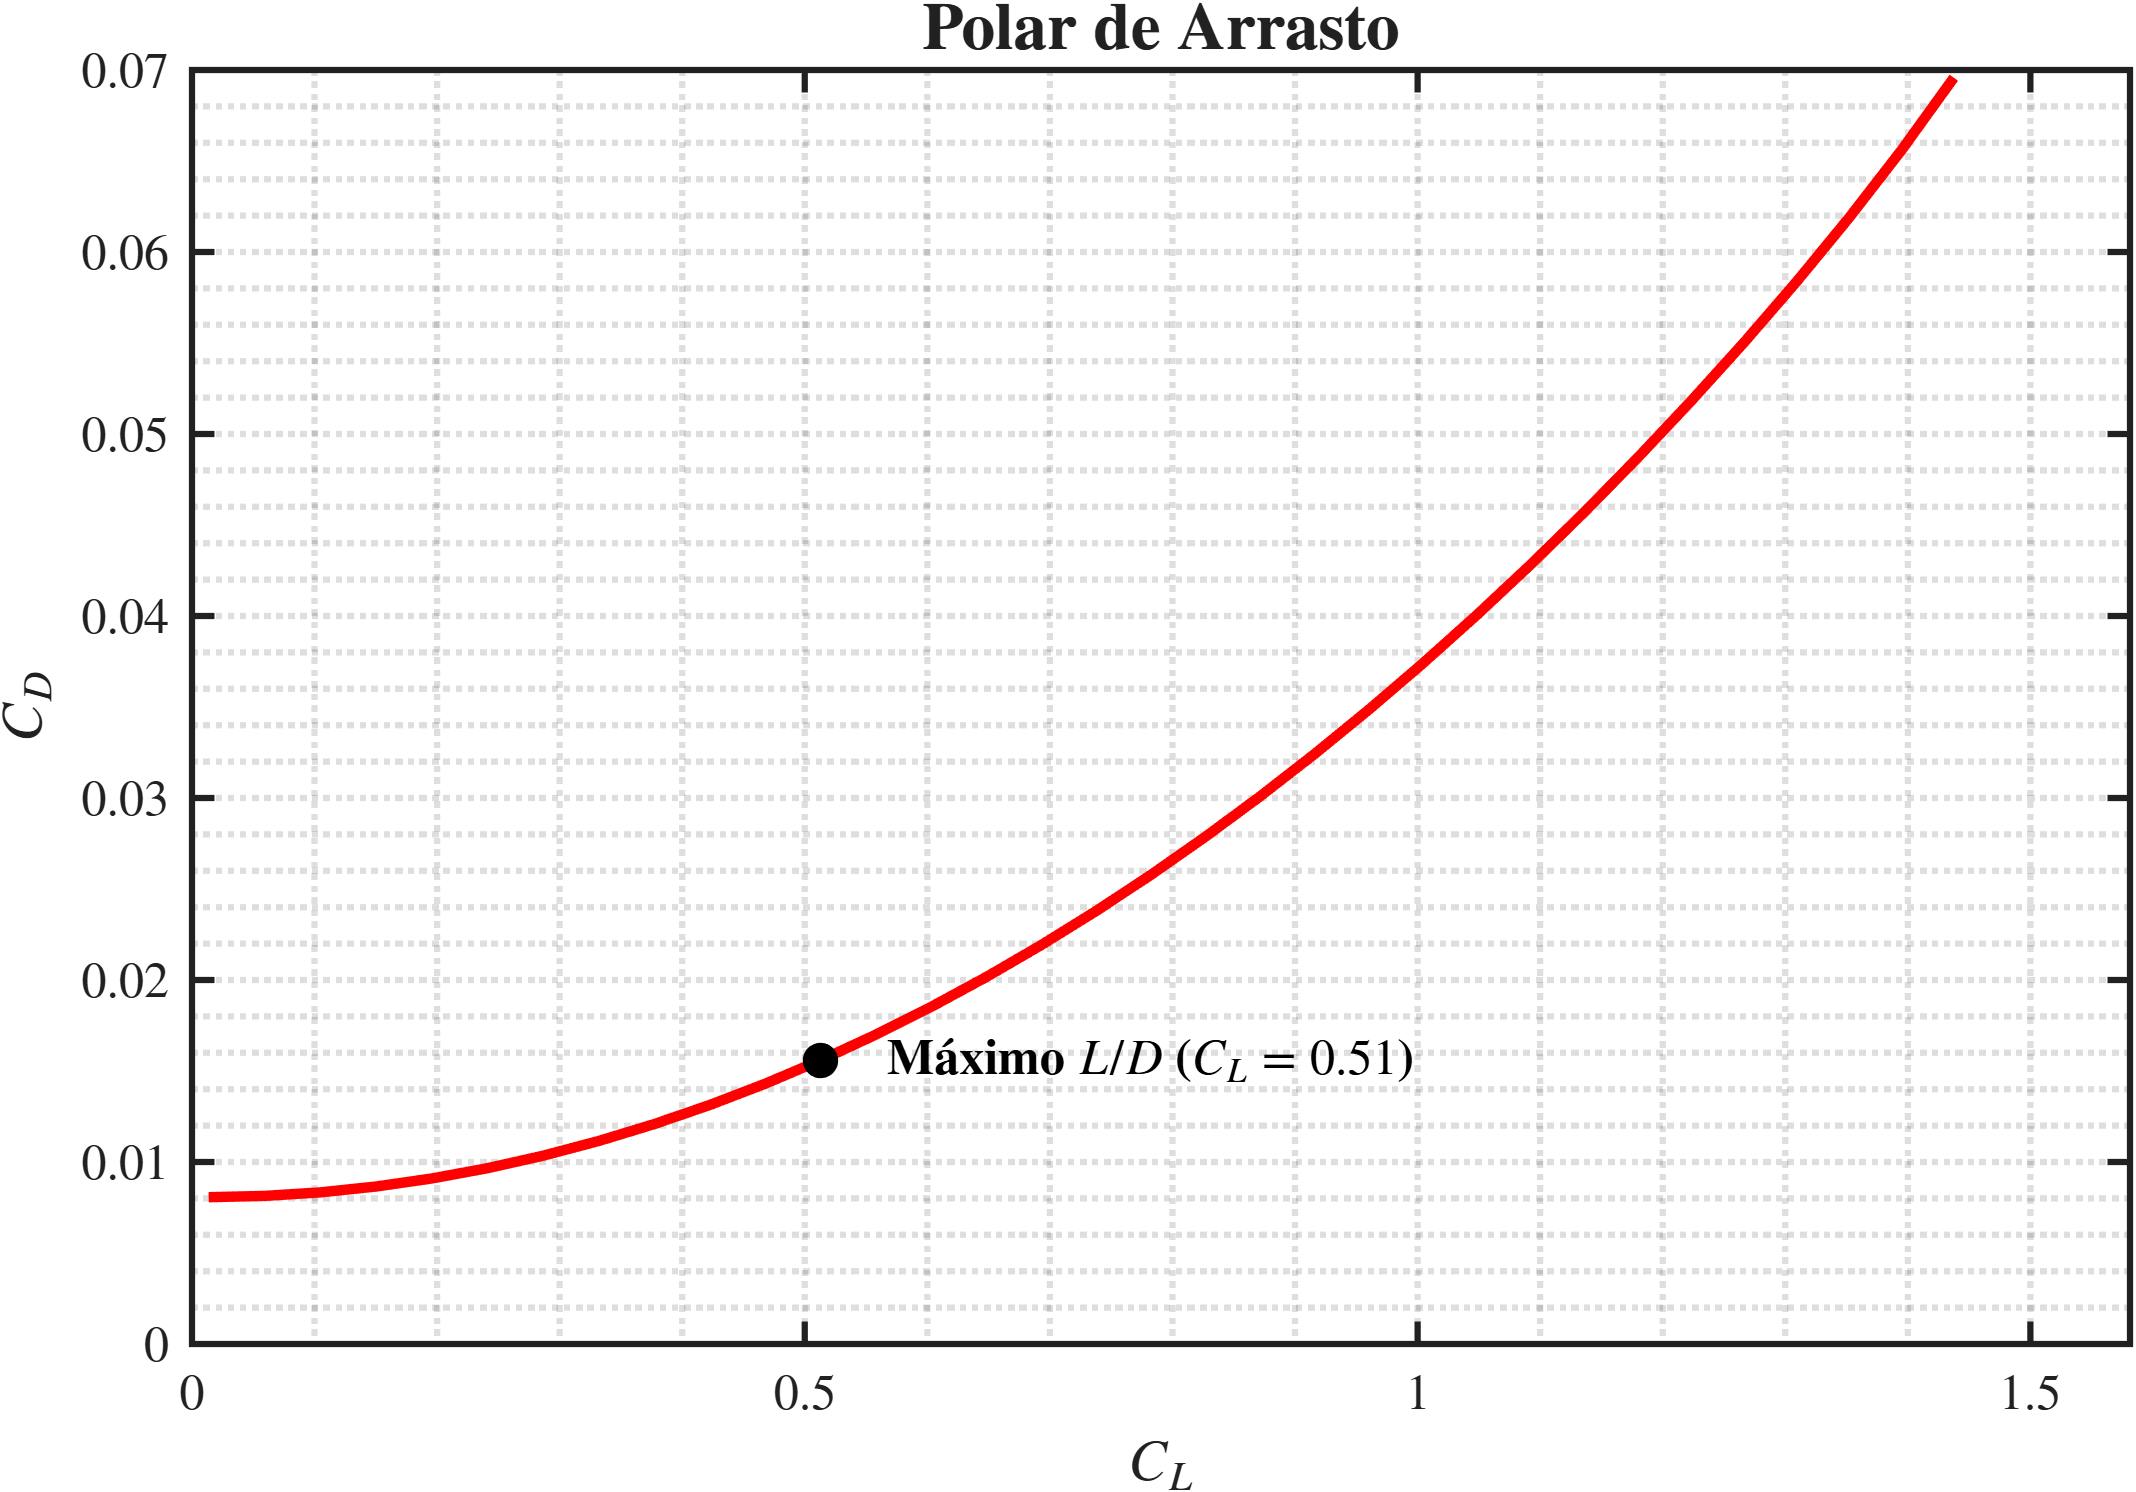
\includegraphics[width=\linewidth]{images/Polar_Arrasto_CL_CD.png}
        \caption{Polar de arrasto da asa ($C_D \times C_L$).}
        \label{fig:polar_arrasto}
    \end{minipage}\hfill
    \begin{minipage}{0.48\textwidth}
        \centering
        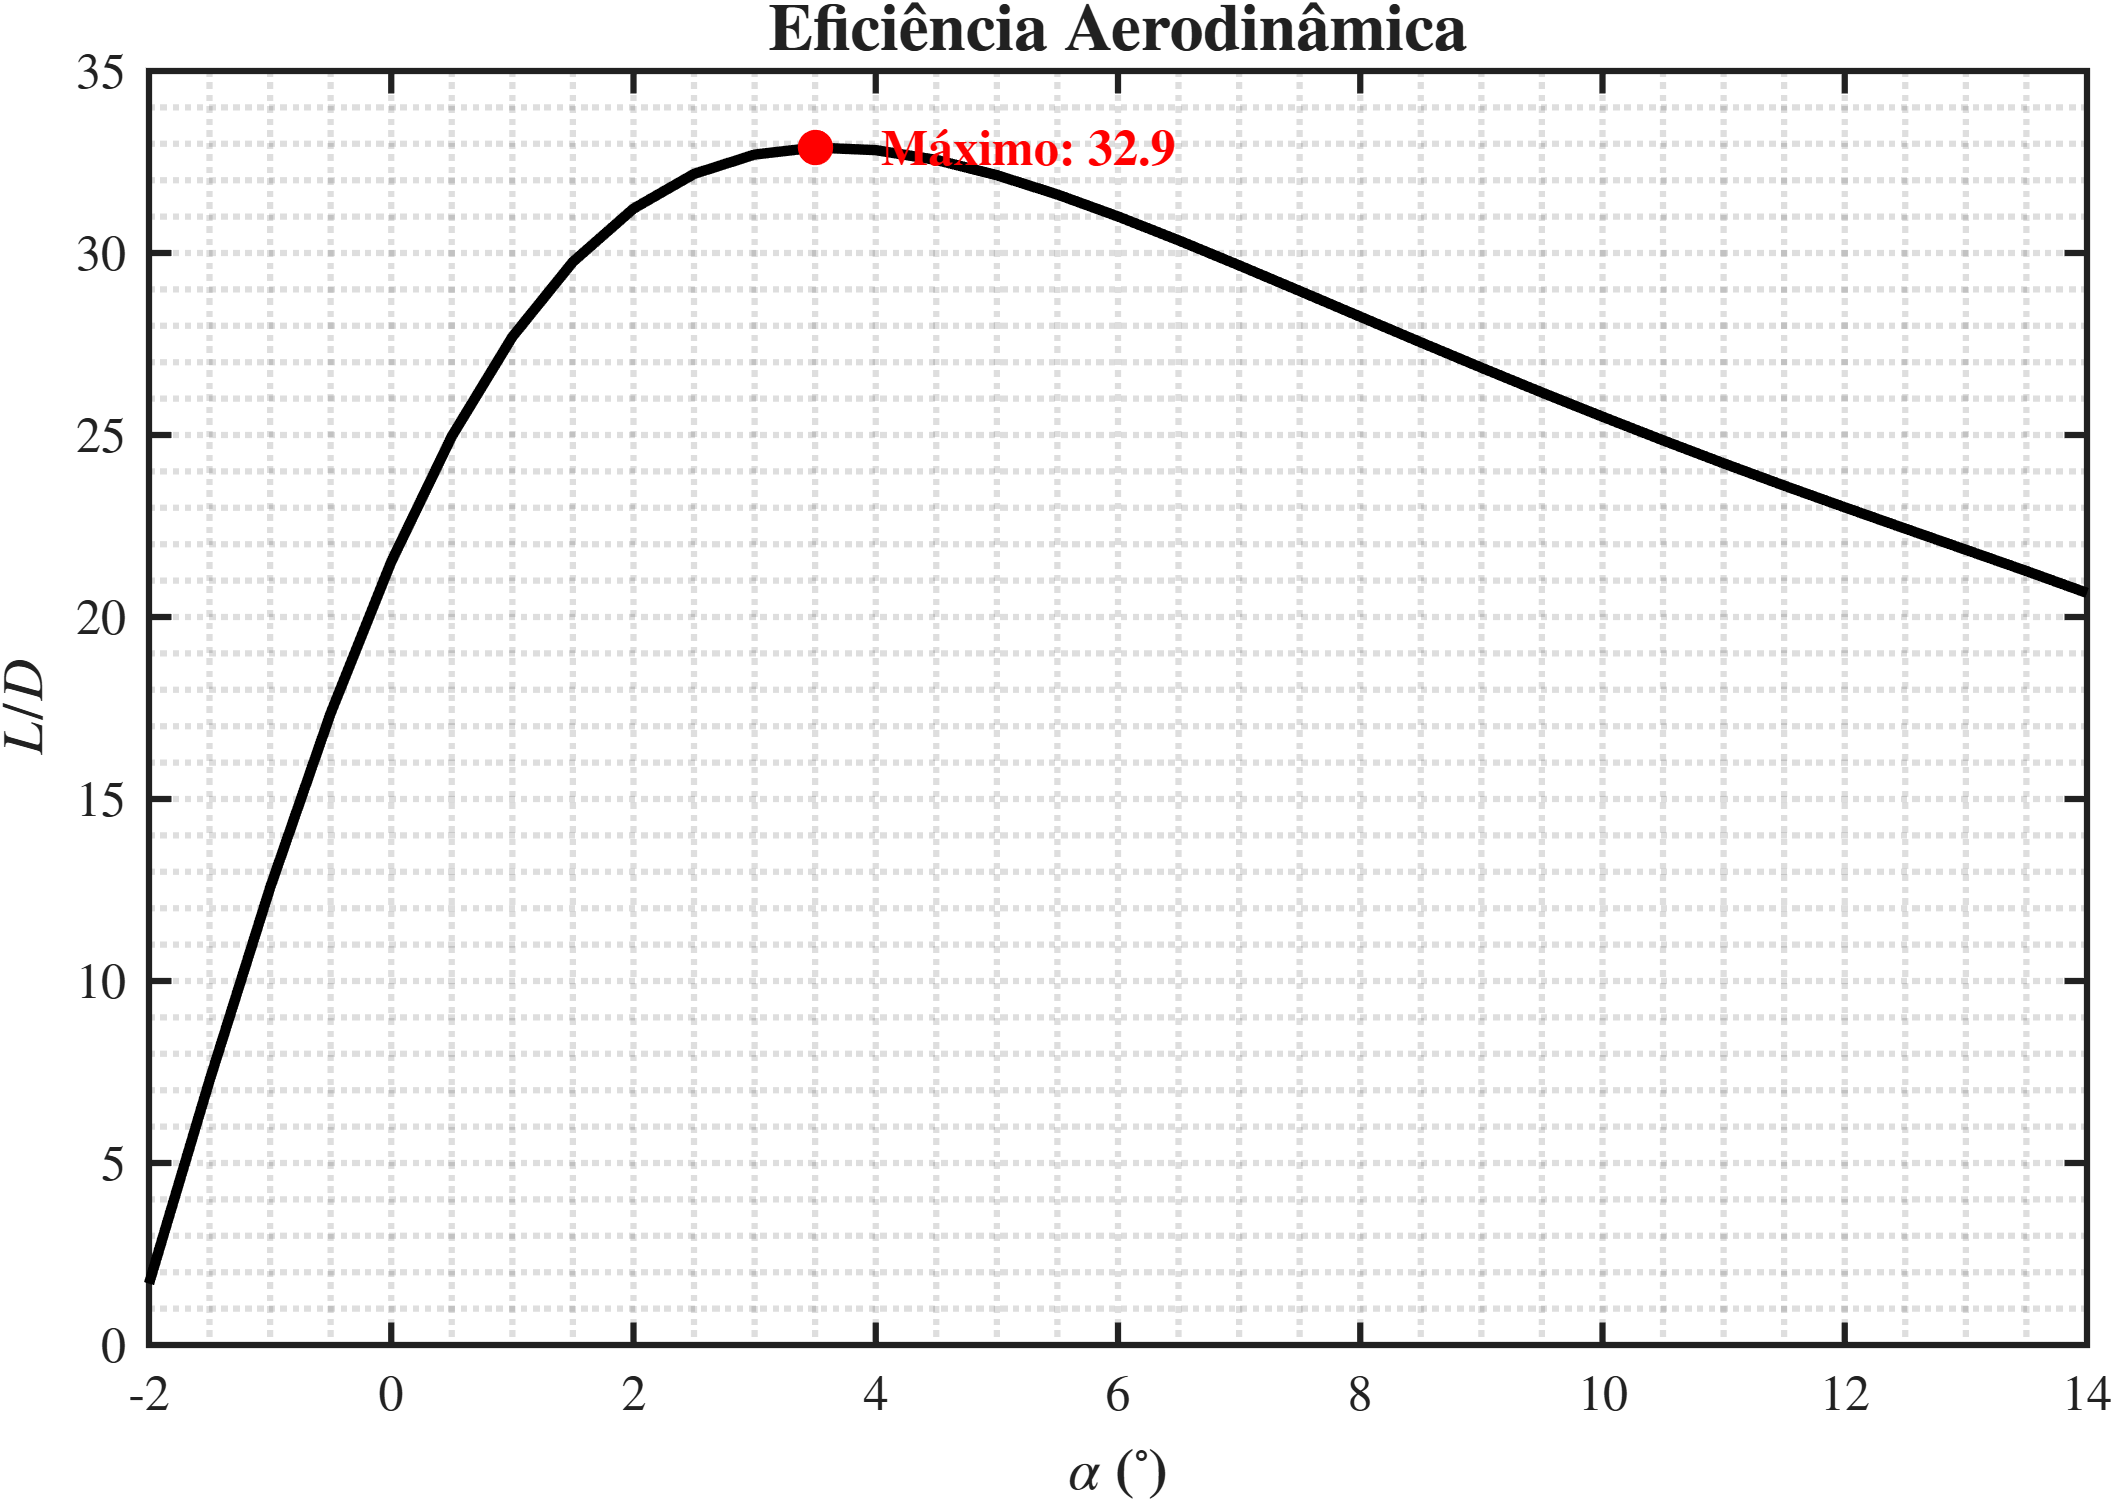
\includegraphics[width=\linewidth]{images/Eficiencia_Aerodinamica.png}
        \caption{Curva de eficiência aerodinâmica ($L/D \times \alpha$).}
        \label{fig:eficiencia_aero}
    \end{minipage}
\end{figure}

A eficiência máxima foi $L/D \approx 32,9$ em $C_L=0,51$, valor próximo ao coeficiente de sustentação de projeto e compatível com a condição de cruzeiro adotada.


\subsection{Dimensionamento dos Flaps}

A determinação do coeficiente de sustentação máximo na configuração limpa,
$C_{L_{\max,\text{limpo}}}$, constitui o ponto de partida para o dimensionamento
do sistema de hipersustentação. Este valor foi obtido por meio de simulação
numérica no software XFLR5, apresentado anteriormente. O resultado desta análise
é apresentado na Figura~\ref{fig:xflr5CLmax}, da qual extrai-se:
 
\begin{equation}
    C_{L_{\max,\text{limpo}}} \approx 1{,}50
\end{equation}
 
\begin{figure}[H]
    \centering
    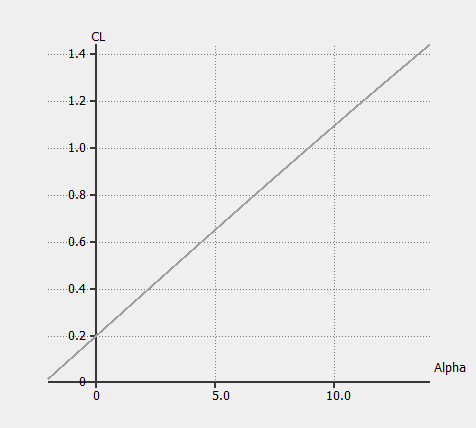
\includegraphics[width=0.50\linewidth]{images/xflr5CLmax.png}
    \caption{Gráfico $C_L$ por $\alpha$ obtido no XFLR5.}
    \label{fig:xflr5CLmax}
\end{figure}

\begin{equation}
\label{eq:CLnormal}
    C_L = \frac{MTOW \cdot g}{\frac{1}{2}\rho V^2 S_{wing}}
\end{equation}

A partir da equação \ref{eq:CLnormal}, adaptada para isolar a velocidade,
conforme a equação \ref{eq:Vestol}:

\begin{equation}
    V_{\text{estol}} = \sqrt{\frac{2W}{\rho\, C_{L_{\max}}\, S}}
    \label{eq:Vestol}
\end{equation}

\noindent encontra-se a velocidade de estol na configuração limpa,
$V_{\text{estol,limpo}} = 111$~kt, correspondente ao $C_{L_{\max,\text{limpo}}} = 1{,}50$
obtido numericamente no XFLR5.

Por meio das análises comparativas com as aeronaves similares apresentadas na
Tabela~\ref{tab:perfiscomparativos}, estabeleceu-se que a velocidade máxima de
estol na configuração com flap é $V_{\text{estol,flap}} = 83$~kt. Aplicando
esta velocidade na equação \ref{eq:CLnormal}, determina-se o coeficiente de
sustentação máximo requerido na configuração com flap:

\begin{equation}
    C_{L_{\max,\text{flap}}} = 2{,}69
    \label{eq:CLmaxflap}
\end{equation}

As velocidades de operação para as fases de decolagem e pouso são definidas
pelo \S~25.107 e \S~25.125 do FAR Part~25~\cite{far25}, que estabelecem
fatores mínimos sobre a velocidade de pouso e decolagem a partir das velocidades de estol do projeto. Para a decolagem, a velocidade de segurança deve satisfazer:

\begin{equation}
    V_{decolagem} \geq 1{,}13 \cdot V_{\text{estol,limpo}}
    \label{eq:vto}
\end{equation}

\noindent e para o pouso, a velocidade deve satisfazer:

\begin{equation}
    V_\text{pouso} \geq 1{,}30 \cdot V_{\text{estol,flaps}}
    \label{eq:vref}
\end{equation}

A partir das equações \ref{eq:CLnormal}, \ref{eq:vto} e \ref{eq:vref}, calculam-se
as velocidades operacionais e os respectivos coeficientes de sustentação, evidenciados na tabela a seguir.

\begin{table}[H]
    \centering
    \caption{Coeficientes de sustentação e velocidades por condição de voo.}
    \label{tab:clmax}
    \begin{tabular}{lcc}
        \toprule
        \textbf{Condição} & \textbf{Velocidade (kt)} & $\boldsymbol{C_L}$ \\
        \midrule
        Estol limpo  (XFLR5)                                       & 111 & 1,50 \\
        Decolagem ($1{,}13\,V_{\text{estol,limpo}}$, \S~25.107) & 125 & 1,17 \\
        Estol com flap (análise comparativa)                 &  83 & 2,69 \\
        Pouso ($1{,}30\,V_{\text{estol,flap}}$, \S~25.125)  & 108 & 1,59 \\
        \bottomrule
    \end{tabular}
\end{table}

\noindent A partir dos valores consolidados na Tabela~\ref{tab:clmax}, verifica-se que
os $C_L$ operacionais de decolagem e pouso se situam no máximo até
 $C_{L_{\max,\text{flap}}} = 2{,}69$,
o que garante a viabilidade do projeto do sistema de hipersustentação. 

Com todos os valores de $C_L$ importantes do projeto explicitados, calcula-se
o incremento de sustentação necessário $\Delta C_{L_{\max}}$ entre a
configuração limpa e a configuração com flap:

\begin{equation}
    \Delta C_{L_{\max}} = C_{L_{\max,\text{flap}}} - C_{L_{\max,\text{limpo}}}
    = 2{,}69 - 1{,}50 = 1{,}19
    \label{eq:deltaCL}
\end{equation}

\noindent Este valor orienta a escolha do tipo de flap mais adequado ao projeto,
uma vez que diferentes dispositivos de hipersustentação produzem incrementos
distintos de $C_{L_{\max}}$. 

Com base na Tabela~12.2 do capítulo 12.4.6 de \cite{raymer2018}, que apresenta
os incrementos típicos de $C_{L_{\max}}$ para diferentes dispositivos de
hipersustentação, optou-se pelo flap \textit{single slotted}, o qual oferece
um incremento máximo de $\Delta C_{L_{\max}} = 1{,}3$. Este valor supera o
incremento requerido pelo projeto de $\Delta C_{L_{\max}} = 1{,}19$,
confirmando que o dispositivo escolhido é capaz de atender aos requisitos
estabelecidos pelo \S~25.107 e \S~25.125 do FAR Part~25~\cite{far25}.

Os ângulos de deflexão adotados para o sistema de flap são de $10^{\circ}$ para a
decolagem e $40^{\circ}$ para o pouso. Estas configurações foram simuladas no XFLR5
utilizando \textit{plain flaps}, uma vez que o simulador não dispõe de modelos
para o flap \textit{single slotted} escolhido. Por ser um dispositivo de menor
eficiência aerodinâmica que o \textit{single slotted}, o \textit{plain flap}
representa apenas uma visualização do incremento de sustentação em operação que deve ser superada.


\begin{figure} [h]
    \centering
    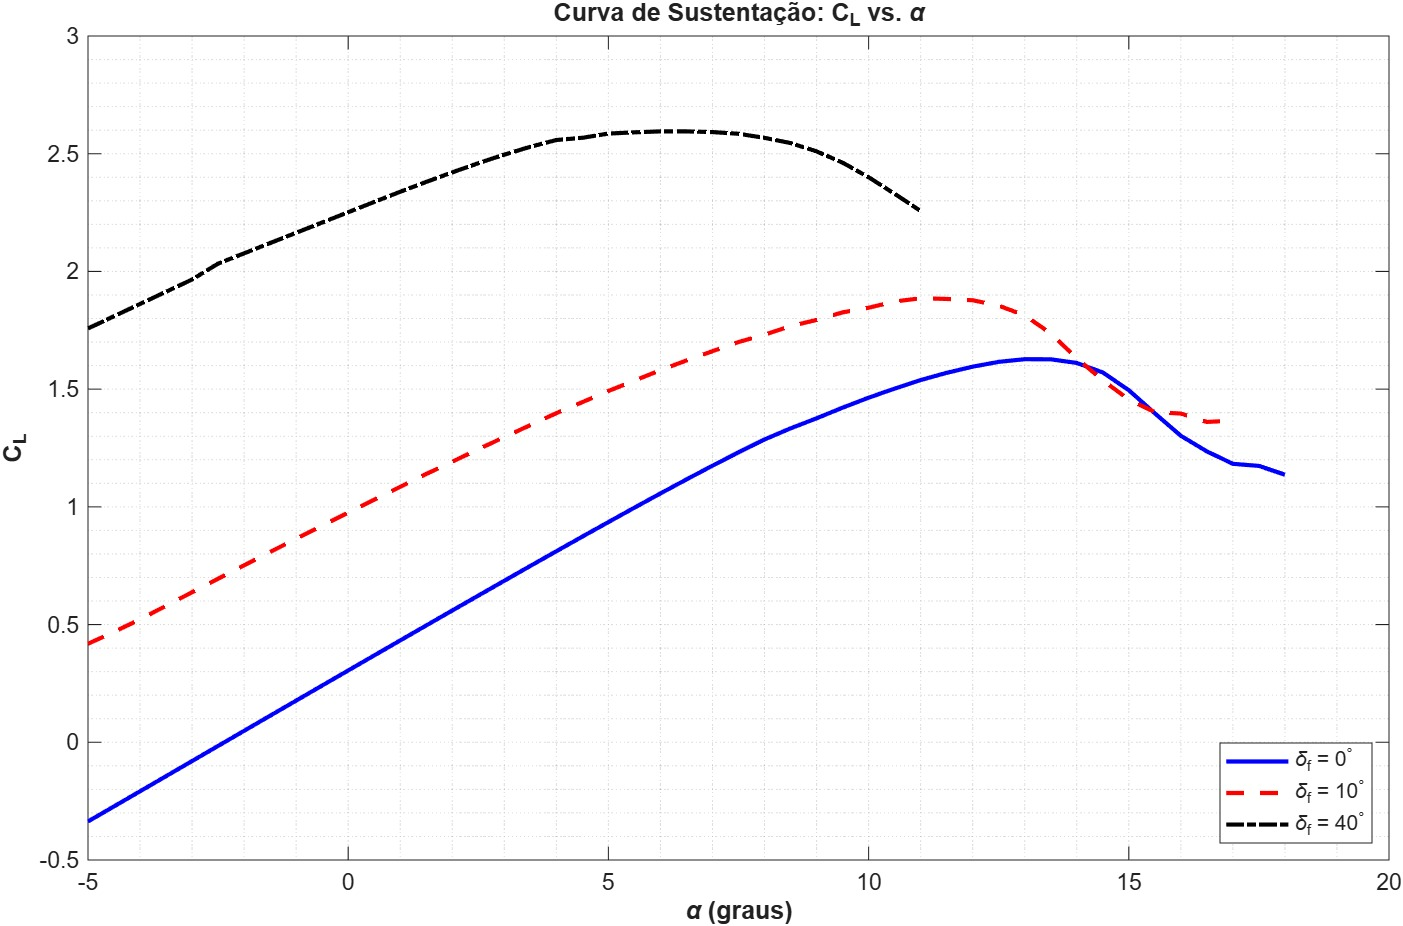
\includegraphics[width=0.8\linewidth]{falpslegais.png}
    \caption{Efeito dos flaps simulados}
    \label{fig:efeito dos flaps}
\end{figure}

\subsection{\textit{Washout}}

Com a forma em planta e os perfis aerodinâmicos previamente definidos, procedeu-se à avaliação da implementação de torção geométrica negativa (\textit{washout}) nas pontas da asa. Esta modificação teve como objetivos principais o incremento da eficiência aerodinâmica global da aeronave, visando otimizar o alcance e minimizar os custos operacionais e o consumo de energia em rota, a atenuação da intensidade dos vórtices de ponta e a redução do momento fletor na raiz por meio da redistribuição do carregamento ao longo da envergadura. Ademais, o \textit{washout} foi projetado para garantir características favoráveis e seguras de estol, induzindo o deslocamento do início do estol para a região entre $33\%b$ e $40\%b$ da semi-envergadura, preservando assim a autoridade de rolamento nas fases críticas de voo \cite{raymer1992}.

\begin{figure}[H]
    \centering
    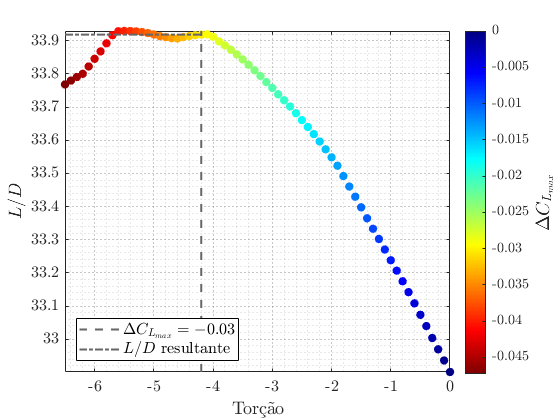
\includegraphics[width=0.7\linewidth]{images/washout_LD.png}
    \caption{Sensibilidade de $\frac{L}{D}$}
    \label{fig:wahsout_LD}
\end{figure}

\begin{figure}[H]
    \centering
    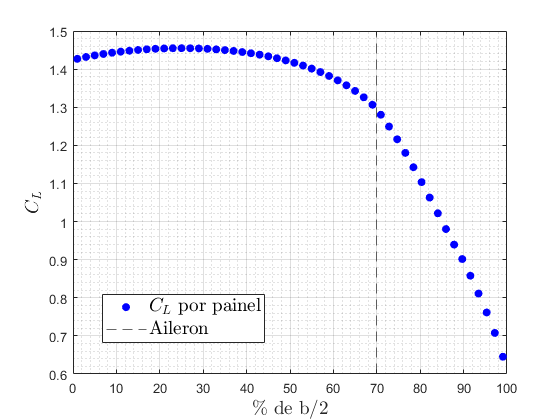
\includegraphics[width=0.7\linewidth]{images/washout_estol.png}
    \caption{Distribuição de $C_L$ por painel}
    \label{fig:washout_estol}
\end{figure}

Como observado na \autoref{fig:wahsout_LD}, a adoção de ângulos de torção muito acentuados acarreta uma degradação geométrica que penaliza o coeficiente de sustentação máximo da asa. Dessa forma, buscando o melhor balanço entre o $L/D$ e $C_{L_{max}}$, adotou-se a maior torção admissível tal que a penalidade no limite de sustentação fosse restrita a $\Delta C_{L_{max}} \geq -0.03$, possibilitanto o ganho de $\Delta \frac{L}{D}_{max} \approx1$.

\section{Geometria das Empenagens e Superficies de Controle}

\subsection{Empenagens Horizontal e Vertical}

O valor dos volumes de cauda definidos no anteprojeto se mantiveram onde: 

\begin{equation*}
    \overline{V}_{HT} = 1,1   \qquad  \overline{V}_{VT} = 0,08
\end{equation*}

A partir dos volumes de cauda e dos valores já definidos de geometria da asa, assim como por meio de análises comparativas já mostradas anteriormente, foram definidas as geometrias das empenagens horizontal e vertical.




\begin{table}[H]
    \centering
    \caption{Geometria da empenagem horizontal}
    \begin{tabular}{c c c c c c c}
    \hline
     $S_{HT}$  & $b_{HT}$ & $c_{r_{HT}}$ & $l_{EH}$ & $\lambda_{HT}$ & $\Gamma_{HT}$ & $\Lambda_{HT}$ \\
     \hline
     18,679 m$^2$ & 8,375 m & 2,788 m & 12,0 m & 0,60 & 0 $\degree$ &  8,5$\degree$ \\
     \hline
    \end{tabular}
    \label{GeoEH_Final}
\end{table}

\begin{table}[H]
    \centering
    \caption{Geometria da empenagem vertical.}
    \begin{tabular}{c c c c c c c}
    \hline
     $S_{VT}$  & $b_{VT}$ & $c_{r_{VT}}$ & $l_{VH}$ & $\lambda_{VT}$ & $\Gamma_{VT}$ & $\Lambda_{VT}$ \\
     \hline
     15,359 m$^2$ & 4,925 m & 4,158 m & 11,0 m & 0,50 & 0 $\degree$ &  25$\degree$ \\
     \hline
    \end{tabular}
    \label{GeoEV_Final}
\end{table}

Para a definição do perfil das empenagens foi realizada a mesma análise de momento e cortante feita na asa, na sessão \ref{analise_espessura}. A força de sustentação da empenagem horizontal foi considerada como sendo a força de balanceamento para voo reto nivelado ao nível do mar. Dessa forma, foi escolhido o perfil simétrico NACA 0012.

\subsection{Superfícies de Controle}

Para o dimensionamento das superfícies de controle, foram novamente utilizados os dados da análise comparativa.

\subsubsection{Profundor}

Para o profundor foi decido que sua corda é constante, com valor igual a 30\% da corda na raiz ($c_r$) do estabilizador horizontal, e cobrindo toda sua envergadura.


\begin{table}[H]
    \centering
     \caption{Dimensões do profundor.}
    \begin{tabular}{c c c}
    \hline
     $S_{\eta}$  & $\overline{c_{\eta}}$ & $b_{\eta}$  \\
     \hline
     5,721 m$^2$ & 0,683 m & 8,375 m \\
      \hline
    \end{tabular}
    \label{Profundor_geo}
\end{table}


\subsubsection{Leme}

Para o leme foi definido que sua corda será constante com valor de 30\% da corda na raiz da empenagem vertical, e também ocupa toda sua envergadura.

\begin{table}[H]
    \centering
     \caption{Dimensões do leme.}
    \begin{tabular}{c c c}
    \hline
     $S_{\zeta}$  & $\overline{c_{\zeta}}$ & $b_{\zeta}$  \\
     \hline
     4,778 m$^2$ & 0,97 m & 4,925 m \\
      \hline
    \end{tabular}
    \label{leme_geo}
\end{table}


\subsubsection{Aileron}

Os ailerons possuem corda constante ao equivalente de 30\% da corda média aerodinâmica, e possuem uma envergadura de 25\% da envergadura da aeronave. Sua posição está mais afastada das asas, a uma distância de 70\% da metade de sua envergadura. As dimensões apresentadas na tabela a seguir já englobam ambos os ailerons direito e esquerdo.

\begin{table}[H]
    \centering
     \caption{Dimensões dos ailerons.}
    \begin{tabular}{c c c}
    \hline
     $S_{\xi}$  & $\overline{c_{\xi}}$ & $b_{\xi}$  \\
     \hline
     5,878 m$^2$ & 0,825 m & 3,563 m \\
      \hline
    \end{tabular}
    \label{ailer_geo}
\end{table}


\section{Geometria interna}

\subsection{Ergonomia}
\label{sec:ergonomia}

O desenvolvimento da cabine de comando foi realizado com base nos requisitos
estabelecidos pela regulamentação de aviação 14 CFR Part 25
(\S 25.771 a \S 25.781), que trata dos aspectos relacionados ao cockpit e à
interação do piloto com os comandos. O requisito 14 CFR Part 25
(\S 25.771) estabelece que a cabine deve permitir operação segura e eficiente
da aeronave, garantindo adequada disposição dos tripulantes e dos comandos.
Já 14 CFR Part 25 (\S 25.773) define requisitos relacionados ao campo de visão
do piloto, exigindo visibilidade adequada durante táxi, decolagem e pouso.
Os requisitos 14 CFR Part 25 (\S 25.777 e \S 25.779) abordam a disposição,
acessibilidade e movimentação dos controles, visando reduzir a possibilidade
de erros operacionais, enquanto 14 CFR Part 25 (\S 25.781) estabelece critérios
para diferenciação tátil e visual das manetes e comandos principais.

Entretanto, a 14 CFR Part 25 apresenta esses requisitos de maneira
predominantemente qualitativa, sem especificar dimensões geométricas fixas
para o dimensionamento da cabine de comando. Dessa forma, para o
desenvolvimento dos desenhos deste projeto, utilizou-se como referência a
aeronave ATR 72-600, por possuir características operacionais e configuração
semelhantes às da aeronave desenvolvida neste trabalho. Em complemento à
geometria do ATR, para garantir o rigor do estudo ergonômico na modelagem no
Fusion 360, foram utilizadas as diretrizes do Human Factors Design Standard
(HFDS) da FAA. Desse documento, extraíram-se principalmente as dimensões
anatômicas estatísticas de pilotos dos sexos masculino e feminino em diferentes
percentis populacionais. A integração dessas duas referências norteou o
posicionamento relativo dos pilotos, a definição da geometria geral do cockpit
e a disposição dos painéis frontal, superior e pedestal central, além da
organização dos comandos de voo, navegação e gerenciamento dos motores.
Dessa maneira, os critérios ergonômicos relacionados ao alcance físico dos
controles, campo de visão do piloto, posicionamento dos displays principais e
separação funcional dos sistemas puderam ser quantificados, buscando atender
plenamente aos requisitos de operação segura, acessibilidade e visibilidade
previstos pela 14 CFR Part 25.

\begin{figure}[H]
    \centering
    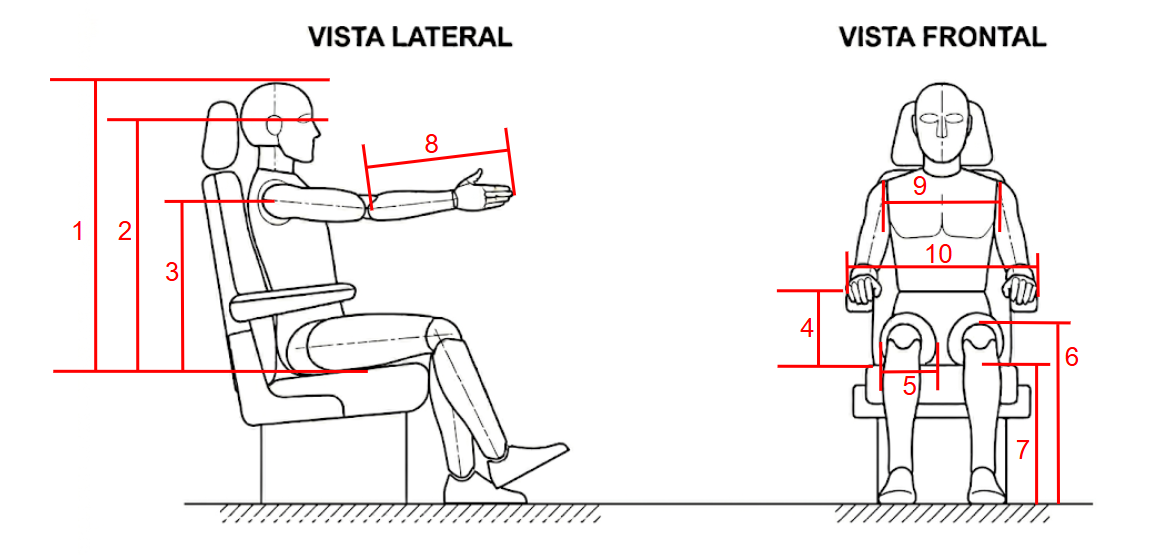
\includegraphics[width=0.60\textwidth]{images/Figura_3_27.png}
    \caption{Esquema de referência para as dimensões ergonômicas da cabine.}
    \label{fig:dimensoes_ergonomicas_cabine}
\end{figure}

\begin{table}[H]
\centering
\caption{Dimensões anatômicas estáticas detalhadas para ergonomia da cabine [cm].}
\label{tab:dimensoes_anatomicas_cabine}
\resizebox{\textwidth}{!}{%
\begin{tabular}{lcccccc}
\hline
\textbf{Dimensão} &
\multicolumn{3}{c}{\textbf{Masculino (M)}} &
\multicolumn{3}{c}{\textbf{Feminino (F)}} \\
\cline{2-7}
& \textbf{5º} & \textbf{50º} & \textbf{95º}
& \textbf{5º} & \textbf{50º} & \textbf{95º} \\
\hline
1 - Altura em posição sentada &
85,8 & 91,4 & 97,2 & 79,5 & 85,1 & 91,0 \\

2 - Altura dos olhos, sentado &
73,5 & 79,2 & 84,8 & 68,5 & 73,8 & 79,4 \\

3 - Altura do ombro, sentado &
54,9 & 59,8 & 64,6 & 50,9 & 55,5 & 60,4 \\

4 - Altura do cotovelo, sentado &
18,4 & 23,2 & 27,4 & 17,6 & 22,1 & 26,4 \\

5 - Espessura da coxa &
14,9 & 16,8 & 19,0 & 14,0 & 15,8 & 18,0 \\

6 - Altura do joelho, sentado &
51,4 & 55,8 & 60,6 & 47,4 & 49,8 & 56,0 \\

7 - Altura poplítea, sentado &
39,5 & 43,3 & 47,6 & 35,1 & 38,9 & 42,9 \\

8 - Comprimento antebraço-ponta do dedo &
44,8 & 48,3 & 52,4 & 40,6 & 44,2 & 48,3 \\

Alcance funcional do braço &
73,9 & 80,0 & 86,7 & 67,7 & 73,4 & 79,7 \\

9 - Largura dos ombros (bideltoide) &
45,0 & 49,1 & 53,5 & 39,7 & 43,1 & 47,2 \\

10 - Largura entre cotovelos &
47,8 & 54,5 & 62,1 & 41,5 & 46,7 & 52,8 \\
\hline
\end{tabular}%
}

\vspace{0.2cm}
\small Fonte: Adaptado de FAA HFDS, Seção 5.12.3.2.
\end{table}

Com base no levantamento das dimensões anatômicas detalhadas e nos requisitos
operacionais preestabelecidos, desenvolveu-se um modelo tridimensional
preliminar da cabine de comando utilizando o software Fusion 360. As figuras
a seguir apresentam os esboços iniciais resultantes dessa modelagem. Por se
tratar de uma concepção conceitual, a geometria e o arranjo apresentados estão
sujeitos a refinamentos e possíveis alterações nas fases subsequentes do projeto.
Contudo, esses modelos já fornecem uma visualização consistente da disposição
espacial interna, elaborada com foco contínuo na ergonomia da tripulação.
O dimensionamento físico das estações de trabalho foi conduzido com o objetivo
de garantir a correta acomodação dos pilotos, assegurando a acessibilidade física
aos comandos e a estrita manutenção dos volumes de tolerância, de modo a evitar
colisões ou restrições de espaço entre os ocupantes e a estrutura da cabine de
piloto. O resultado está apresentado nas imagens a seguir:

\begin{figure}[H]
    \centering
    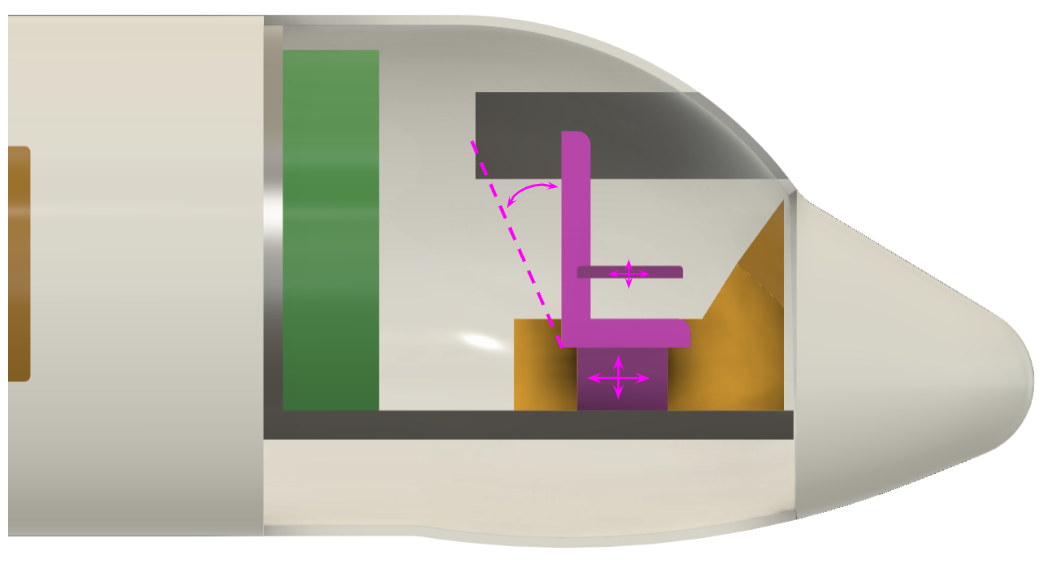
\includegraphics[width=0.70\textwidth]{images/Figura_3_28.png}
    \caption{Visão geral do arranjo ergonômico preliminar da cabine de comando.}
    \label{fig:arranjo_ergonomico_cabine}
\end{figure}

\begin{figure}[H]
    \centering
    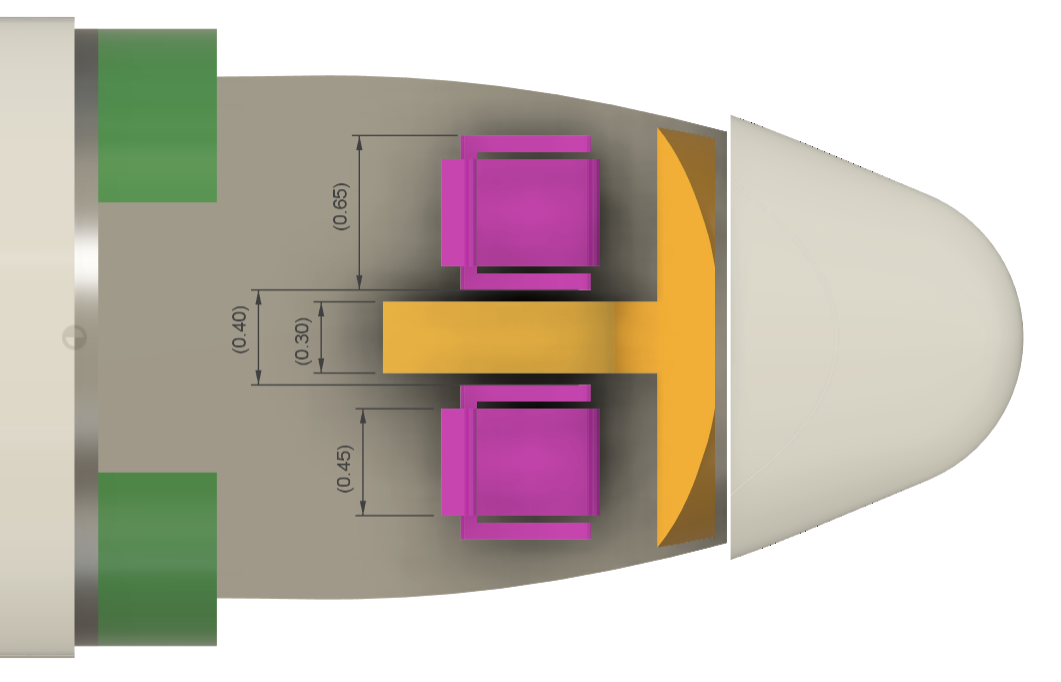
\includegraphics[width=0.70\textwidth]{images/Figura_3_29.png}
    \caption{Vista superior da disposição espacial.}
    \label{fig:vista_superior_cabine}
\end{figure}

\begin{figure}[H]
    \centering
    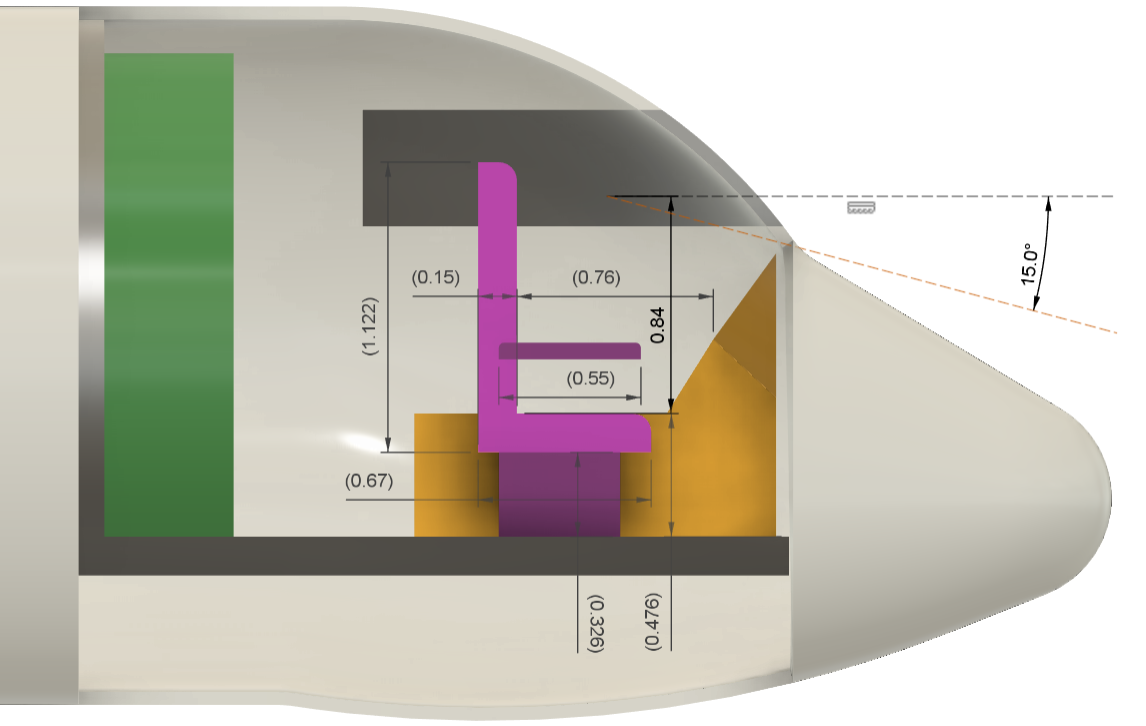
\includegraphics[width=0.70\textwidth]{images/Figura_3_30.png}
    \caption{Vista lateral do assento da tripulação de comando.}
    \label{fig:vista_lateral_assento}
\end{figure}

\subsection{Painel de Comando e Aviônicos}
\label{sec:painel_comando_avionicos}

A aeronave é certificada sob RBAC~25~\cite{rbac25}, FAR Part~25~\cite{far25} e
CS-25~\cite{cs25}, incluindo os requisitos associados à disposição dos
instrumentos e comandos no painel. O requisito determinante para o
\textit{layout} é o CS/FAR-25.1321, que estabelece critérios para o agrupamento
e posicionamento dos instrumentos de voo em relação ao plano vertical da visão
frontal do piloto. A disposição das informações primárias segue o conceito
denominado \textit{basic T}, herdado da instrumentação eletromecânica clássica
e mantido nos \textit{glass cockpits} por meio da representação gráfica
equivalente no \textit{Primary Flight Display} (PFD)~\cite{cs25,skybrary_pfd}.

Dessa forma, adota-se uma configuração \textit{glass cockpit} integrada,
compatível com o estado da arte em aeronaves turboélice regionais e tendo como
referência a arquitetura empregada no ATR 72-600. A escolha em detrimento da
instrumentação eletromecânica permite concentrar as principais informações de
voo, navegação, motorização e sistemas em displays eletrônicos, reduzindo a
quantidade de instrumentos individuais e favorecendo a integração das
informações apresentadas aos pilotos.

A disposição do painel é definida de forma integrada aos critérios
antropométricos apresentados na seção anterior. Seu posicionamento considera a
posição dos olhos dos pilotos, a linha normal de visada, o alcance funcional dos
membros superiores e a necessidade de preservar a visibilidade externa da
cabine. Dessa forma, busca-se manter as informações essenciais à condução da
aeronave no campo primário de visão e garantir adequada acessibilidade aos
comandos.

Na cabine de comando, mais especificamente no painel, são disponibilizadas aos
pilotos informações necessárias à aeronavegabilidade por meio dos aviônicos,
``equipamentos eletrônicos ou de processamento de dados utilizados para
controle, comunicação e/ou navegação em aeronaves'', segundo definição da
ANAC.

A instrumentação e equipamentos mínimos necessários para operação da aeronave é
estabelecida por meio do regulamento brasileiro de aviação civil e depende da
categoria da aeronave e dos equipamentos instalados, a exemplo do motor
utilizado. Desse modo, o RBAC~25 Subparte F~\cite{rbac25} determina que para
motores turboélice os seguintes equipamentos são necessários:

\begin{itemize}
    \item Indicador de combustível individual para cada motor;
    \item Alarmes de falhas/avisos;
    \item Indicador de óleo;
    \item Indicador de pressão de óleo para cada motor individual;
    \item Indicador de temperatura de óleo;
    \item ``Alarme'' de incêndio;
    \item Medidor de quantidade de fluído;
    \item Indicador de \textit{cooler} dos motores;
    \item Indicador de torque individual;
    \item Indicador para ângulo de pá de hélice;
    \item Meio para monitoramento do sistema de fluídos.
\end{itemize}

Outrossim, para que a aeronave possa operar a qualquer horário do dia e não
dependa exclusivamente da visibilidade dos pilotos, devem ser considerados os
instrumentos e equipamentos para voo IFR, estabelecidos no
RBAC~91~\cite{rbac91}. Portanto, é possível citar entre os principais
equipamentos:

\begin{itemize}
    \item Indicador de velocidade do ar;
    \item Um altímetro;
    \item Um indicador de direção que apresente a proa magnética;
    \item Ao menos um rádio-comunicação bilateral VHF, incluindo fones e
    microfones associados, caso o voo ou o espaço aéreo exija radiocomunicação
    bilateral contínua;
    \item Ao menos um equipamento de rádio-navegação apropriado a cada estação
    solo, quando o tipo de voo ou espaço aéreo requerer radionavegação;
    \item Um indicador giroscópico de atitude (horizonte artificial);
    \item Um indicador giroscópico de direção (giro direcional ou equivalente).
\end{itemize}

Destaca-se que a regulamentação exige equipamentos além dos citados para voo
IFR, mas parte foi omitida no presente relatório em razão da extensão da lista.

Para a operação em geral, considerando que a aeronave projetada é de categoria
\textit{commuter}, também é exigido pelo RBAC~91 o uso de um transponder, um
sistema de percepção e alarme de proximidade do solo (TAWS) e dois transmissores
localizadores de emergência (ELT), um do tipo automático e outro do tipo
portátil ou de sobrevivência, flutuante e à prova d'água.

Por fim, as demandas quanto aos equipamentos elétricos da aeronave incluem dois
sistemas independentes de fonte, dois sistemas de rádio comunicação e rádio
navegação independente. Ademais, o RBAC~25 Subparte F estabelece que sistemas
essenciais devem contar com alguma via de fonte extra, a fim de assegurar seu
funcionamento caso haja falha na via principal.

Além disso, é reforçado que a alocação dos componentes elétricos deve ser feita
de modo a minimizar o risco, a exemplo do requerimento para cablagem, cuja
instalação deve ser conforme demanda de corrente e de modo a não provocar
interferências, a fim de evitar curto-circuito.


\subsubsection{Configuração do painel de comando}

A configuração do painel é organizada de maneira aproximadamente simétrica em
relação ao eixo longitudinal da aeronave, permitindo que comandante e copiloto
tenham acesso direto às informações necessárias à condução do voo. Adota-se um
conjunto de cinco \textit{Display Units} (DU), distribuídas da esquerda para a
direita da seguinte forma:

\begin{itemize}
    \item DU 1 e DU 5: correspondem aos
    \textit{Primary Flight Displays} (PFD) do comandante e do copiloto,
    respectivamente. Apresentam as informações primárias necessárias à condução
    da aeronave, incluindo atitude, velocidade, altitude, velocidade vertical e
    direção, mantendo a organização digital equivalente ao conceito
    \textit{basic T};

    \item DU 2 e DU 4: correspondem aos
    \textit{Multi-Function Displays} (MFD), destinados à apresentação de
    informações complementares de navegação e dos sistemas da aeronave,
    incluindo informações provenientes do radar meteorológico, TAWS e TCAS;

    \item DU 3: corresponde ao sistema central de indicação dos
    parâmetros dos motores e alerta à tripulação, EICAS
    (\textit{Engine Indication and Crew Alerting System}). Sua posição central
    permite visualização pelos dois pilotos e possibilita a apresentação
    conjunta dos parâmetros dos dois motores, bem como das mensagens de alerta
    associadas aos sistemas da aeronave.
\end{itemize}

A adoção dessa arquitetura mantém duas unidades de PFD e duas unidades de MFD,
uma para cada posto de pilotagem, acrescentando uma unidade central destinada
ao monitoramento dos motores e sistemas. Dessa forma, as informações primárias
de voo permanecem diretamente associadas a cada piloto, enquanto informações
de interesse comum podem ser apresentadas na região central do painel.

Entre os displays centrais é previsto um Sistema Integrado de Instrumentos de
Reserva (IESI), destinado a disponibilizar informações essenciais de voo em
caso de indisponibilidade dos displays principais. Sua localização na região
central favorece a visualização por ambos os pilotos e acrescenta uma camada
independente de redundância à instrumentação principal.

A disposição física preliminar dos principais elementos da cabine de comando é
apresentada na Figura~\ref{fig:painel_frontal}. O arranjo evidencia a distribuição
simétrica dos cinco displays principais, constituídos pelos dois PFDs, dois MFDs
e pelo EICAS central, além da posição do IESI, do \textit{glareshield}, do
pedestal central e do painel \textit{overhead}. A configuração busca manter as
informações primárias diretamente associadas aos respectivos postos de pilotagem,
enquanto os sistemas e comandos compartilhados são posicionados em regiões
acessíveis a ambos os pilotos.

\begin{figure}[H]
    \centering
    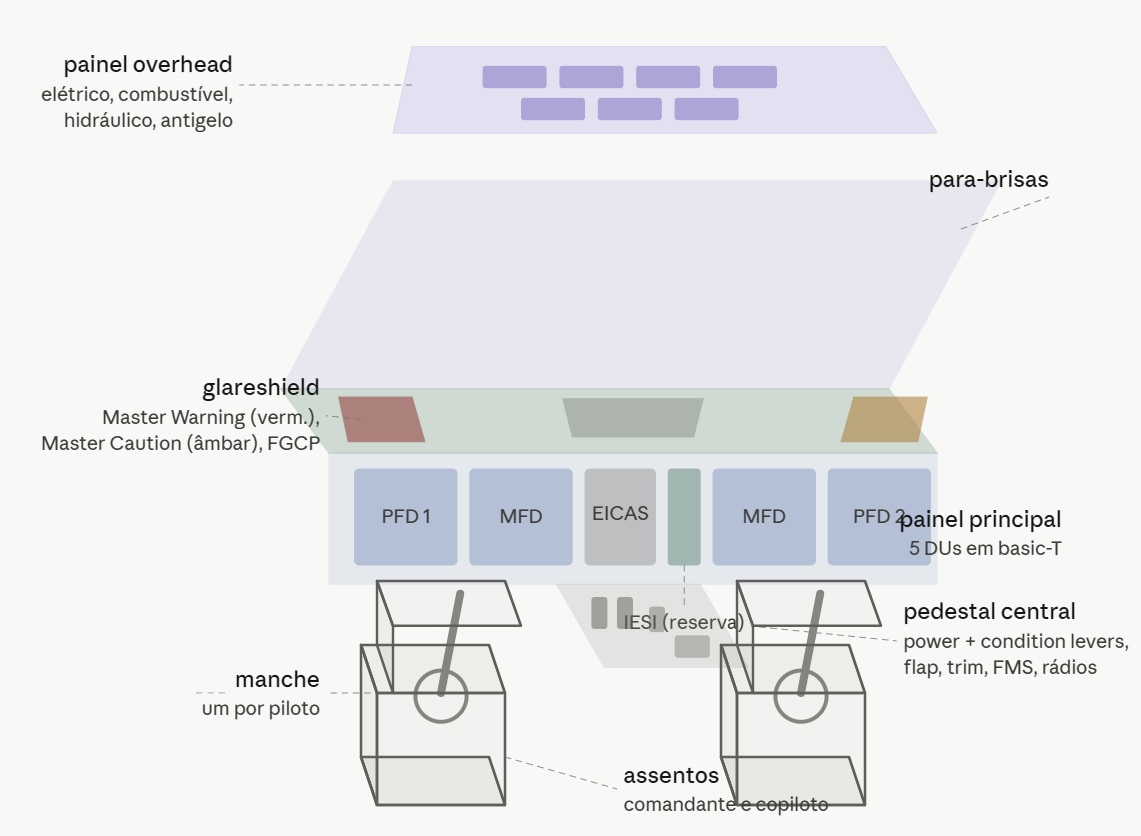
\includegraphics[width=0.75 \linewidth]{esbocopainel.png}
    \caption{Esboço inicial da disposição do painel de instrumentos.}
    \label{fig:painel_frontal}
\end{figure}

A Figura~\ref{fig:integracao_avionicos} apresenta, de forma complementar, a
arquitetura funcional dos principais sistemas aviônicos da aeronave,
evidenciando o fluxo de informações até sua apresentação aos pilotos. As
representações de PFD e MFD nessa arquitetura correspondem às respectivas
funções de apresentação, enquanto sua implementação física no painel é realizada
por dois PFDs e dois MFDs, além do EICAS central.

\begin{figure}[H]
    \centering
        \includegraphics[width=0.9\linewidth]{Figura_3_31.png}
    \caption{Integração dos sistemas de aviônica.}
    \label{fig:integracao_avionicos}
\end{figure}

O PFD constitui a principal interface para apresentação das informações
necessárias à condução da aeronave. Nele são concentrados os parâmetros
fundamentais de voo, permitindo ao piloto acompanhar simultaneamente as
condições de atitude, velocidade, altitude e direção. A concentração dessas
informações mantém a lógica de apresentação associada ao \textit{basic T},
porém em formato digital e integrado.

A Figura~\ref{fig:pfd} apresenta as principais informações que, de acordo com
os requisitos considerados, devem ser disponibilizadas aos pilotos no
\textit{Primary Flight Display}.

\begin{figure}[H]
    \centering
    \includegraphics[width=0.85\linewidth]{Figura_3_32.png}
    \caption{Informações principais do PFD.}
    \label{fig:pfd}
\end{figure}

Os MFDs complementam as informações apresentadas nos PFDs, possibilitando a
visualização de dados de navegação e informações provenientes dos demais
sistemas da aeronave. Essa divisão permite manter os parâmetros fundamentais de
voo permanentemente disponíveis nos PFDs, enquanto informações complementares
podem ser selecionadas e apresentadas nos MFDs conforme a necessidade
operacional.


\subsubsection{Distribuição funcional dos comandos}

Além dos displays principais, o painel de comando é dividido funcionalmente
entre painel frontal, \textit{glareshield}, pedestal central e painel
\textit{overhead}. Essa divisão permite organizar os comandos de acordo com sua
importância operacional, frequência de utilização e necessidade de acesso pela
tripulação.

O \textit{glareshield}, localizado imediatamente acima do painel principal,
acomoda os comandos relacionados ao sistema de orientação de voo e piloto
automático, permitindo sua operação sem grande afastamento da linha de visada
principal. Nessa região também são posicionados os anunciadores de
\textit{Master Warning} e \textit{Master Caution}, permitindo rápida
identificação visual de condições que demandem atenção da tripulação.

O pedestal central, localizado entre os assentos dos pilotos, agrupa os comandos
compartilhados entre os dois postos de pilotagem. Para a configuração
turboélice, são dispostos nessa região os comandos associados aos motores e
hélices, incluindo \textit{power levers} e \textit{condition levers}, além dos
comandos de \textit{flaps}, compensadores e das unidades relacionadas ao
gerenciamento de voo, comunicação e navegação.

Adicionalmente, devido ao fato de o painel ser composto quase integralmente por
displays, com exceção de alguns equipamentos, como a MCDU
(\textit{Multipurpose Control Display Unit}) --- localizada na região inferior
entre os pilotos ---, a unidade \textit{clock}, o sistema ELVE SET
(\textit{Landing Elevation}), entre outros, tais instrumentos são integrados às
regiões funcionais do painel de acordo com sua frequência de utilização e
necessidade de acesso.

O painel \textit{overhead}, por sua vez, aloja principalmente comandos
associados aos sistemas que não necessitam permanecer continuamente no campo
primário de visão dos pilotos, incluindo os sistemas elétrico, hidráulico,
combustível, pressurização, antigelo e partida. Dessa forma, o painel frontal
permanece prioritariamente destinado às informações diretamente relacionadas à
condução e monitoramento do voo.

A organização conjunta dessas regiões busca reduzir a dispersão dos comandos,
facilitar sua identificação e manter as informações e controles de maior
importância operacional nas regiões de melhor visualização e alcance.


\subsubsection{Integração com a ergonomia da cabine}

As dimensões críticas e a posição do painel são estabelecidas a partir dos
critérios antropométricos apresentados na seção anterior. A posição nominal dos
olhos dos pilotos constitui uma referência para a determinação da altura e da
inclinação do painel, bem como para o posicionamento dos displays principais.

A linha normal de visada considerada na análise ergonômica encontra-se
aproximadamente $15^{\circ}$ abaixo da horizontal. Dessa forma, o posicionamento
dos displays principais busca manter as informações de maior relevância
operacional próximas à região natural de visualização dos pilotos, reduzindo a
necessidade de movimentos excessivos da cabeça durante a leitura dos
instrumentos.

Simultaneamente, a borda superior do painel deve preservar o campo de visão
externo através dos para-brisas. A posição do painel, dos olhos dos pilotos e
dos para-brisas é, portanto, considerada de maneira conjunta, de modo a
compatibilizar a leitura dos instrumentos com a visibilidade necessária durante
as operações de táxi, decolagem, aproximação e pouso.

O alcance dos comandos também é relacionado às dimensões antropométricas
adotadas para a cabine. Os comandos de utilização frequente devem permanecer
dentro do alcance funcional dos pilotos na posição normal de operação, enquanto
a distribuição entre painel frontal, \textit{glareshield}, pedestal e
\textit{overhead} deve evitar interferências entre os ocupantes e permitir
acesso adequado aos diferentes sistemas.


\subsubsection{Seleção dos principais equipamentos aviônicos}

Foi realizada uma pesquisa entre modelos de aviônicos comumente
empregados nessa categoria de aeronave, os quais, em sua maioria, possuem
arquitetura remota --- sendo instalados no compartimento de aviônicos da
aeronave. A Tabela~\ref{tab:modelos_avionicos} apresenta alguns dos modelos
encontrados e sugeridos por fabricantes consolidados no mercado, os quais
atendem aos requisitos de certificação TSO e DO-160 necessários para aplicação
aeronáutica.

\begin{table}[H]
    \centering
    \caption{Modelos de aviônicos sugeridos para a aeronave.}
    \label{tab:modelos_avionicos}
    
    \renewcommand{\arraystretch}{1.25}
    \setlength{\tabcolsep}{6pt}
    
    \begin{tabular}{|p{0.24\textwidth}|p{0.18\textwidth}|p{0.19\textwidth}|p{0.30\textwidth}|}
        \hline
        
        \textbf{Equipamento} &
        \textbf{Fabricante} &
        \textbf{Modelo} &
        \textbf{Observação} \\
        \hline
        
        Função VOR/VHF/TCAS &
        Garmin &
        GTN 725 &
        Possui certificação para aplicações em aeronaves ATR 72, podendo ser uma opção para diminuir displays ou ser integrado como \textit{standby}. \\
        \hline
        
        Transponder &
        ACSS &
        NTX-600 &
        Utilizado no ATR e com aplicação comprovada para categoria da aeronave. \\
        \hline
        
        FMS 1 e 2 &
        Thales Group &
        FMS-220 &
        Utilizado no ATR. \\
        \hline
        
        Sistema Radar &
        Honeywell Aerospace &
        RDR-400 &
        Utilizado no EMB-190, que possui aviônicos em comum com o EMB-170. \\
        \hline
        
        Radar Altimeter &
        Honeywell Aerospace &
        KRA-405B com filtro RFF-100 &
        O KRA-405B é o modelo utilizado no EMB-170. O filtro RFF-100 foi uma modificação aprovada para uma aeronave e tem como função reduzir a interferência pelo 5G. \\
        \hline
        
        VOR/ILS &
        Collins &
        VIR-32 &
        Comumente utilizado em muitas aeronaves. \\
        \hline
        
    \end{tabular}
\end{table}


\section{Dimensionamento de Pneus e Freios}
As diretrizes de dimensionamento adotadas baseiam-se nos requisitos de aeronavegabilidade estabelecidos pelo 14 CFR Part 25 da FAA e pelo RBAC 25, aplicáveis a aeronaves de transporte. Para isso, foram adotadas as metodologias de projeto aeronáutico propostas por Daniel P. Raymer e Snorri Gudmundsson, que estão em conformidade com esses requisitos.

\subsection{Distribuição de Cargas no Trem de Pouso}
\label{sec:distribuicao_cargas_tdp}

A distribuição de cargas entre o trem de pouso principal (\textit{Main Landing Gear} - MLG) e o trem de nariz (\textit{Nose Landing Gear} - NLG) é determinada a partir do equilíbrio estático de forças na aeronave. Em configurações triciclo convencionais, o trem de pouso principal suporta aproximadamente 90\% do peso da aeronave, enquanto o de nariz suporta os 10\% restantes.

Para o dimensionamento preliminar, adotou-se essa distribuição de 90\% da carga no MLG e 10\% no NLG, considerando a condição crítica de peso máximo de decolagem (\textit{Weight Takeoff} --- WTO). Conforme recomendado por Raymer e Gudmundsson para aeronaves certificadas sob o FAR Part 25, foi aplicada uma margem adicional de 7\% sobre as cargas estáticas, associada às condições operacionais no solo.  Destaca-se que, apesar de os autores também proporem uma margem de $25 \%$ que pode ser aplicada ao cálculo da cagra máxima, esta é indicada apenas para acrescentar uma folga para possíveis acréscimos de massa na aeronave ao longo de seu dewsenvolvimento. Como este projeto adota o peso máximo de decolagem como pré-requisito, esta margem adicional não se faz necessária. A formulação utilizada para determinação das cargas críticas, então, é dada por:

\begin{equation}
W_{MLG} = \eta_{MLG} \cdot W_{TO} \cdot (1 + \sigma_{FAR}) \cdot (1 + \sigma_{growth})
\end{equation}

\begin{equation}
W_{NLG} = \eta_{NLG} \cdot W_{TO} \cdot (1 + \sigma_{FAR}) \cdot (1 + \sigma_{growth})
\end{equation}

Onde:

\begin{itemize}
    \item $W_{TO} = 50000\ \text{lb}$: peso máximo de decolagem da aeronave;
    
    \item $\eta_{MLG} = 0,90$: fração de carga suportada pelo trem principal;
    
    \item $\eta_{NLG} = 0,10$: fração de carga suportada pelo trem de nariz;
    
    \item $\sigma_{FAR} = 0,07$: margem adicional recomendada para condições operacionais no solo;
    
    \item $\sigma_{growth} = 0,05$: margem de crescimento estrutural.
\end{itemize}

Substituindo os valores adotados nas Equações anteriores, obtêm-se as cargas críticas de projeto para os trens de pouso principal e de nariz:

\begin{equation}
W_{MLG} = 0,90 \cdot 50000 \cdot 1,07 = 48150\ \text{lb} \approx 21840\ \text{kgf}
\end{equation}

\begin{equation}
W_{NLG} = 0,10 \cdot 50000 \cdot 1,07 = 5350\ \text{lb} \approx 2427\ \text{kgf}
\end{equation}

O trem de pouso principal é composto por duas pernas, cada uma equipada com rodas duplas, totalizando quatro pneus ($N_{MLG}=4$). Essa configuração reduz a carga individual por pneu e, consequentemente, a pressão aplicada sobre o pavimento, além de facilitar o alojamento interno do conjunto.

O trem de nariz é constituído por uma única perna com rodas duplas, totalizando dois pneus ($N_{NLG}=2$), configuração adotada para aumentar a estabilidade direcional e a redundância operacional durante as operações em solo.

A partir dessas configurações, determina-se a carga estática atuante em cada pneu individual, considerando as margens de projeto adotadas. Os resultados são apresentados na \autoref{tab:carregamento}.

\begin{table}[H]
    \centering
    \caption{Condições de carregamento do trem de pouso.}
    \vspace{0.2cm}

    \resizebox{\textwidth}{!}{%
    \begin{tabular}{lcccc}
        \toprule
        \textbf{Condição de} & \textbf{Carga Total} & \textbf{Carga Individual} & \textbf{Carga Total} & \textbf{Carga Individual} \\
        \textbf{Carregamento} & \textbf{no MLG (lb/kgf)} & \textbf{por Pneu do MLG (lb/kgf)} & \textbf{no NLG (lb/kgf)} & \textbf{por Pneu do NLG (lb/kgf)} \\
        \midrule
        
        Estática Nominal ($W_{TO}$) 
        & 45000 / 20412 
        & 11250 / 5103 
        & 5000 / 2268 
        & 2500 / 1134 \\
        
        Com Margem FAR Part 25 (+7\%) 
        & 48150 / 21840 
        & 12037,5 / 5460 
        & 5350 / 2427 
        & 2675 / 1213 \\
        
        \bottomrule
    \end{tabular}
    }

    \label{tab:carregamento}
\end{table}


\subsection{Metodologia de Dimensionamento Estatístico}

Antes da seleção definitiva dos pneus a partir de catálogos comerciais, utilizou-se o método estatístico proposto por Raymer \cite{raymer2018} para estimativa preliminar das dimensões dos pneus em aeronaves de transporte civil. O método correlaciona o diâmetro externo ($D_{ext}$) e a largura ($W_{ext}$) do pneu com a carga máxima suportada por roda ($W_w$), em libras.

As correlações utilizadas são:

\begin{equation}
D_{ext} = 1,63 \cdot \left(W_w\right)^{0,315}
\end{equation}

\begin{equation}
W_{ext} = 0,1043 \cdot \left(W_w\right)^{0,480}
\end{equation}

Para o trem de pouso principal, considerando a carga crítica estática com margem regulamentar do FAR Part 25 e sem margem de crescimento estrutural, obtém-se:

\begin{equation}
W_w = \frac{48150}{4} = 12037,5\ \text{lb}
\end{equation}

Substituindo nas Equações anteriores:

\begin{equation}
D_{ext,MLG} = 1,63 \cdot (12037,5)^{0,315}
= 31,54\ \text{in} \approx 801\ \text{mm}
\end{equation}

\begin{equation}
W_{ext,MLG} = 0,1043 \cdot (12037,5)^{0,480}
= 9,48\ \text{in} \approx 240,7\ \text{mm}
\end{equation}

% Considerando também a margem de crescimento estrutural de 25\%:

% \begin{equation}
% W_w = \frac{60.187,5}{4} = 15.046,9\ \text{lb}
% \end{equation}

% \begin{equation}
% D_{ext,MLG} = 1,63 \cdot (15.046,9)^{0,315}
% = 33,81\ \text{in} \approx 859\ \text{mm}
% \end{equation}

% \begin{equation}
% W_{ext,MLG} = 0,1043 \cdot (15.046,9)^{0,480}
% = 10,55\ \text{in} \approx 268\ \text{mm}
% \end{equation}

Para o trem de nariz, considerando a carga crítica estática com margem regulamentar:

\begin{equation}
W_w = \frac{5350}{2} = 2675\ \text{lb}
\end{equation}

\begin{equation}
D_{ext,NLG} = 1,63 \cdot (2675)^{0,315}
= 19,47\ \text{in} \approx 495\ \text{mm}
\end{equation}

\begin{equation}
W_{ext,NLG} = 0,1043 \cdot (2675)^{0,480}
= 4,62\ \text{in} \approx 117\ \text{mm}
\end{equation}


\subsection{Seleção e Especificações de Pneus Comerciais}

Com o objetivo de manter comunalidade com aeronaves da mesma categoria operacional, especialmente o ATR 72, realizou-se a seleção preliminar dos pneus a partir do catálogo da Goodyear Aviation.

Para o trem de pouso principal, optou-se pela utilização de pneus do tipo radial, devido à menor massa estrutural, maior vida útil em ciclos de pouso e melhor desempenho térmico durante frenagens severas.

Para o trem de nariz, selecionou-se um pneu do tipo diagonal (\textit{bias-ply}) equipado com defletor de spray integrado (\textit{chine tire}), solução amplamente empregada em aeronaves turboélice de asa alta para reduzir a projeção de água, detritos e granizo em direção às entradas de ar dos motores durante operações em pista molhada.

\begin{table}[H]
    \centering
    \caption{Especificações dos pneus selecionados para o trem de pouso.}
    \vspace{0.2cm}
    
    \footnotesize
    \setlength{\tabcolsep}{4pt}
    
    \begin{tabular}{p{5.2cm}cc}
        \toprule
        \textbf{Parâmetro Técnico do Fabricante} & \textbf{MLG} & \textbf{NLG} \\
        \midrule
        Tamanho do Pneu (Designação) & H34x10.0R16 & 450x190-5 \\
        Tipo de Construção do Pneu & Radial (Flight Radial) & Diagonal (Flight Leader com Chine) \\
        Part Number (Goodyear) & 346Q48-4 & 459M08-2 \\
        Ply Rating (PR) & 14 & 10 \\
        Carga Homologada (lb/kgf) & 13400 / 6078 & 3822 / 1734 \\
        Pressão Nominal (psi) & 130 & 90 \\
        Diâmetro Máximo Grown (in/mm) & 32,95 / 837 & 17,70 / 450 \\
        Largura Máxima Grown (in/mm) & 9,35 / 237 & 7,50 / 190 \\
        Raio Estático LSD (in/mm) & 14,00 / 356 & 7,05 / 179 \\
        Velocidade Limite (mph / kt) & 190 / 165 & 190 / 165 \\
        Roda / Flange (in) & 16,0 / 7,00 & 5,0 \\
        \bottomrule
    \end{tabular}
    
    \label{tab:pneus_selecionados}
\end{table}


Ainda segundo Raymer \cite{raymer2018}, a pressão operacional dos pneus pode ser ajustada para valores calculados proporcionalmente à pressão nominal em situações de operação abaixo da carga nominal, de modo que:

\begin{equation}
    P_{op}= P_{nom}\frac{W_{op}}{W_{nom}}
\end{equation}

Assim, considerando-se uma pressão nominal de 130 psi, carga operacional de 11250 lb e carga nominal de 13400 lb para o MLG, enquanto esses respectivos valores são de 90 psi, 2500 lb e 3822 lb para o NLG, calcula-se pressões operacionais de 109,15 psi e 58,9 psi para os pneus do trem de pouso principal e de nariz, respectivamente. 

\subsubsection{Análise Comparativa e Validação Física}
Ao comparar os pneus selecionados com as estimativas preliminares obtidas pelo método de Raymer, observa-se boa concordância entre os valores calculados e os dados de catálogo. O pneu principal selecionado apresenta diâmetro externo de 32,95 in, correspondendo a um desvio de aproximadamente +4,5\% em relação ao valor estimado de 31,54 in. A largura nominal de 9,35 in difere em aproximadamente -1,0\% da estimativa de 9,45 in.

A capacidade de carga homologada do pneu H34x10.0R16, igual a 13400 lb, atende à carga regulamentar por roda de 12037,5 lb com margem de aproximadamente 11,3\%.

\subsection{Análise Física do Flanco do Pneu e Operabilidade}

A escolha da geometria do flanco (altura lateral da borracha) constitui um compromisso crítico de projeto entre eficiência aerodinâmica e capacidade de amortecimento no solo. A altura do flanco ($H$) é obtida pela equação:

\begin{equation}
H = \frac{D_{\max} - D_{rim}}{2}
\end{equation}

Onde $D_{\max}$ é o diâmetro externo Grown e $D_{rim}$ é o diâmetro nominal da roda (aro).

\subsubsection*{Pneu Principal (H34x10.0R16)}

\begin{equation}
H_{MLG} = \frac{(32,95 - 16,0)}{2} = 8,475 \ \text{in} \ (\approx 215,3 \ \text{mm})
\end{equation}

A relação de aspecto do flanco em relação à largura do pneu é:

\begin{equation}
\zeta_{MLG} = \frac{H_{MLG}}{w} = \frac{8,475}{9,35} \approx 0,906 \ (90,6\%)
\end{equation}

\subsubsection*{Pneu de Nariz (450x190-5)}

\begin{equation}
H_{NLG} = \frac{(17,70 - 5,0)}{2} = 6,35 \ \text{in} \ (\approx 161,3 \ \text{mm})
\end{equation}

A relação correspondente é:

\begin{equation}
\zeta_{NLG} = \frac{H_{NLG}}{w} = \frac{6,35}{7,50} \approx 0,847 \ (84,7\%)
\end{equation}

A manutenção de uma alta relação de aspecto do flanco ($\zeta > 80\%$) reflete a orientação de projeto estabelecida nesse trabalho para operação em pistas semi-preparadas ou com revestimentos asfálticos deteriorados de aeródromos regionais. O pneu de perfil alto funciona como um sistema secundário de absorção de choque pneumático. Sob impactos verticais causados por detritos ou buracos na pista, a grande deflexão do flanco distribui as forças, reduzindo o estresse dinâmico de pico transmitido à estrutura de fixação do trem de pouso na fuselagem e mitigando os efeitos de fadiga.

Em contrapartida, pneus de perfil baixo e flanco curto, comuns em jatos comerciais rápidos, são projetados estritamente para altas velocidades e pistas perfeitamente lisas, pois minimizam o arrasto e os movimentos de inclinação lateral nas curvas (\textit{rolling stiffness}), porém transmitem impactos de forma severa para a estrutura da aeronave.

A pressão de inflação nominal do pneu do trem principal de $115 \ \text{psi}$ e do trem de nariz de $90 \ \text{psi}$ classifica a aeronave na faixa de pressão intermediária, adequada para operações em pistas de asfalto ou concreto de média resistência, mantendo excelente coeficiente de atrito.


\subsection{Dimensionamento e Análise dos Freios}

\subsubsection{Determinação da Velocidade de Decisão de Decolagem ($V_1$)}

O dimensionamento térmico e mecânico do sistema de freios deve ser conduzido com base
no cenário crítico de \textbf{Decolagem Rejeitada} ($R_{TO}$),
conforme prescrito pelo parágrafo § 25.735(f)(2) do RBAC~25. Nessa condição, a aeronave
se encontra no seu \textbf{Peso Máximo de Decolagem} (MTOW) e a frenagem de emergência
é iniciada na velocidade de decisão $V_1$, que é inerentemente superior à velocidade de
toque de pouso convencional. Por esse motivo, o RTO representa o caso de carregamento
crítico que dita a capacidade térmica mínima do conjunto freio--roda.

A velocidade de decisão de decolagem $V_1$ é estimada de forma conservadora em:

\begin{equation}
    V_1 = 105 \ \text{kt}
\end{equation}

Este valor é compatível com o envelope operacional de decolagem da aeronave de
referência ATR~72-600 (cujo $V_2 \approx 116\ \text{kt}$) e representa uma estimativa
conservadora para projeto preliminar. Convertendo para o sistema imperial:

\begin{equation}
    V_1 = 105 \times 1{,}68781 \approx 177{,}22 \ \text{ft/s}
\end{equation}


\subsubsection{Cálculo da Energia Cinética de Frenagem — Caso $R_{TO}$}

A capacidade térmica mínima do sistema de freios é determinada a partir da energia
cinética total que os freios devem absorver integralmente durante uma parada de
emergência em RTO. Adota-se a condição mais conservadora, sem contribuição de
empuxo reverso nem de arrasto aerodinâmico.

A energia cinética total da aeronave no instante de início da frenagem é dada por:

\begin{equation}
    KE_{total} =
    \frac{1}{2}
    \left(
        \frac{W_{TO}}{g}
    \right)
    V_1^{\,2}
\end{equation}

Onde:

\begin{equation}
    W_{TO} = 50\,000 \ \text{lb}
\end{equation}

\begin{equation}
    g = 32{,}174 \ \text{ft/s}^2
\end{equation}

\begin{equation}
    V_1 = 177{,}22 \ \text{ft/s}
\end{equation}

Substituindo os valores:

\begin{equation}
    KE_{total} =
    \frac{1}{2}
    \left(
        \frac{50\,000}{32{,}174}
    \right)
    (177{,}22)^2
\end{equation}

\begin{equation}
    KE_{total}
    \approx
    24\,379\,000 \ \text{ft-lbf}
\end{equation}

Considerando quatro rodas freadas no trem de pouso principal:

\begin{equation}
    N_{freios} = 4
\end{equation}

A energia cinética absorvida por cada conjunto de freio é:

\begin{equation}
    KE_{roda} =
    \frac{KE_{total}}{N_{freios}}
    =
    \frac{24\,379\,000}{4}
\end{equation}

\begin{equation}
    KE_{roda}
    \approx
    6\,094\,750 \ \text{ft-lbf}
\end{equation}

Convertendo para Joules ($1\ \text{ft-lbf} = 1{,}35582\ \text{J}$):

\begin{equation}
    KE_{roda}
    = 6\,094\,750 \times 1{,}35582
    \approx 8\,263\,000 \ \text{J}
\end{equation}

\begin{equation}
    \boxed{KE_{roda} \approx 8{,}26 \ \text{MJ}}
\end{equation}

Adota-se portanto $KE_{projeto} = 8{,}26\ \text{MJ}$ como capacidade térmica mínima
por conjunto freio--roda para o dimensionamento do sistema de freios, em conformidade
com o caso crítico regulatório de Decolagem Rejeitada exigido pelo § 25.735(f)(2)
do RBAC~25.

\subsection{Seleção da Tecnologia de Freios}

A dissipação de aproximadamente $8,26, \ \text{MJ}$ por roda impõe elevada solicitação térmica ao sistema de frenagem, exigindo materiais com alta resistência térmica e estabilidade estrutural. Para a aeronave, adotou-se o uso de freios multidisco de carbono em substituição aos conjuntos convencionais de aço.

As principais características e impactos dessa escolha são apresentados na \autoref{tab:comparacao_freios}.

\begin{table}[H]
    \centering
    \caption{Comparação entre tecnologias de freios aeronáuticos.}
    \vspace{0.2cm}

    \renewcommand{\arraystretch}{1.6}
    \setlength{\tabcolsep}{6pt}

    \begin{tabular}{|p{3.5cm}|p{3.2cm}|p{3.5cm}|p{5.2cm}|}
        \hline
        \textbf{Propriedade / Característica} &
        \textbf{Freios de Aço} &
        \textbf{Freios de Carbono} &
        \textbf{Impacto Técnico no Projeto} \\
        \hline

        Peso do Conjunto de Freios
        & Elevado (referência)
        & Redução de 35\% a 42\% em massa
        & Redução do OEW e aumento da capacidade de carga paga ou combustível \\
        \hline

        Condutividade Térmica
        & Moderada
        & Elevada
        & Dissipação térmica mais eficiente e menor risco de superaquecimento \\
        \hline

        Resistência Térmica e Vida Útil
        & Perda de eficiência acima de $500^\circ$C; vida útil entre 800 e 1200 ciclos
        & Operação estável até $1200^\circ$C; vida útil entre 1500 e 3000 ciclos
        & Maior confiabilidade operacional e redução de manutenção \\
        \hline

        Custo de Aquisição Inicial
        & Baixo
        & Elevado
        & Maior custo inicial compensado pela durabilidade e menor custo operacional \\
        \hline
    \end{tabular}

    \label{tab:comparacao_freios}
\end{table}


\subsection{Sistema de Atuação Hidráulica e Segurança}

O acionamento do trem de pouso e do sistema de freios é realizado por um sistema hidráulico operando a $3.000 \ \text{psi}$, alimentado por bombas acopladas à caixa de acessórios dos motores PW127M. A arquitetura hidráulica é dividida em circuitos redundantes para atendimento aos requisitos de segurança do RBAC 25.

\begin{itemize}
    \item \textbf{Circuito Hidráulico Primário de Retração e Frenagem:} responsável pelo acionamento dos atuadores de recolhimento do trem de pouso e pelo fornecimento de pressão hidráulica às pinças de freio do trem principal, com sistema anti-skid.

    \item \textbf{Circuito Hidráulico Secundário:} atua automaticamente em caso de falha do circuito primário, mantendo capacidade residual de frenagem e esterçamento do trem de nariz.

    \item \textbf{Extensão de Emergência por Gravidade:} em caso de perda total de pressão hidráulica, o sistema libera os mecanismos de travamento superior (\textit{uplocks}), permitindo a extensão do trem de pouso por gravidade e arrasto aerodinâmico, com travamento mecânico na posição abaixada.
\end{itemize}

\subsection{Geometria de Alojamento do Trem de Pouso em Asa Alta}

Na configuração de asa alta, o recolhimento do trem principal diretamente para o interior da asa exigiria o comprimento do trem de pouso excessivamente grande, aumentando peso e momentos fletores quando em contato com o solo. Para evitar essa limitação, o trem principal é fixado às estruturas inferiores da fuselagem e recolhido lateralmente para carenagens externas do tipo \textit{sponson}, solução utilizada em aeronaves como ATR 72 e CASA C-295.

Esse arranjo apresenta as seguintes vantagens:

\begin{itemize}
    \item preservação da caixa de torção da asa (\textit{wing box}) para cargas aerodinâmicas e armazenamento de combustível;

    \item redução do comprimento das pernas do trem de pouso e, consequentemente, da massa estrutural do sistema;

    \item simplificação do mecanismo de retração hidráulica por rotação lateral com travamento por tesoura.
\end{itemize}

O trem de nariz é recolhido para a região frontal da fuselagem, abaixo do cockpit. O recolhimento para frente favorece o travamento aerodinâmico em caso de falha hidráulica.

\subsection{Posicionamento do trem de pouso}
\label{sec:posicionamento_tdp}

\subsubsection{Comprimentos}

Pelo FAR Part 25, há a exigência de que a hélice esteja a pelo menos $7"$ do solo, ou 178 mm. Com isso, a partir da clearance lateral exigida, conforme Trahmer, na figura \ref{fig:lateral clearence} e pela geometria, foi possível estimar uma altura de 0,70 m para os trens de pouso, considerando que a aeronave ficará nivelada em solo.

\begin{figure}[H]
    \centering
    \begin{minipage}{0.8\textwidth} % Ajuste o 0.8 para aumentar ou diminuir o tamanho
        \centering
        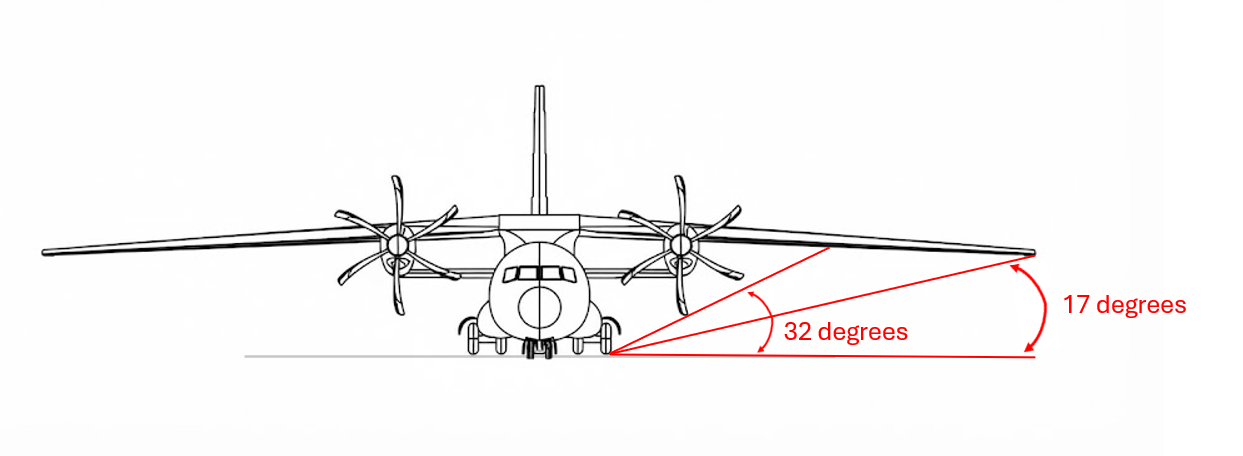
\includegraphics[width=\linewidth]{images/Altura aeronave.png}
        \caption{Requeirmento de clearance lateral}
        \label{fig:lateral clearence}
    \end{minipage}
\end{figure}

\subsubsection{Posicionamento}

Os componentes do trem de pouso têm que ser posicionados de forma a evitar que a aeronave tombe ao realizar manobras em solo. Isso é feito de forma a posicionar cada perna em relação ao CG, de 10,82 m a partir do nariz e de 0,59 m a partir do ponto mais baixo da fuselagem.

Naturalmente, o NLG, por ser constituido de apenas uma perna, é posicionado na linha de simetria da aeronave.
A partir do requerimento de ângulo de turnover mostrado na figura \ref{fig:trem lateral} e o CG vertical de 0,59 m, é possível apontar que a bitola fica em torno de 4,1 m.

\begin{figure}[H]
    \centering
    \begin{minipage}{0.8\textwidth} % Ajuste o 0.8 para aumentar ou diminuir o tamanho
        \centering
        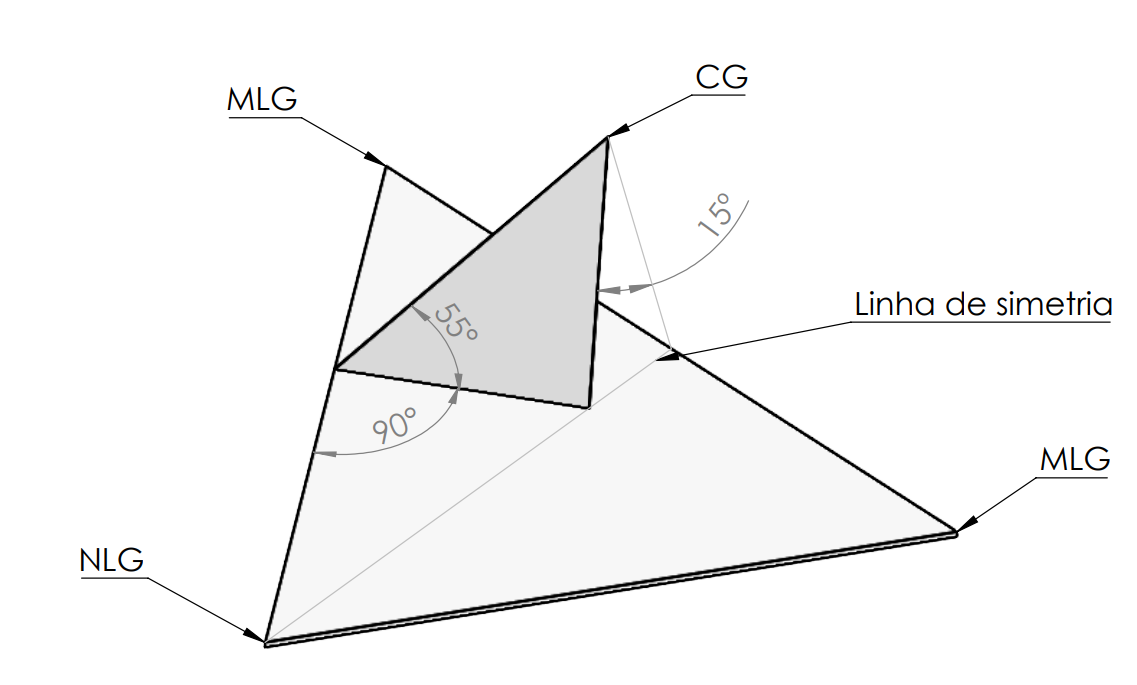
\includegraphics[width=\linewidth]{images/Posição lateral do trem de pouso.png}
        \caption{Posição lateral do trem de pouso.}
        \label{fig:trem lateral}
    \end{minipage}
\end{figure}

Já em relação ao posicionamento longitudinal, o trem de pouso de nariz foi arbitrariamente posicionado a 1,87 m do nariz. Esse valor vem da análise comparativa e corrobora com a estrutura interna da aeronave, ajustado posteriormente com base no avanço do projeto.

Já o trem de pouso principal deve estar posicionado de forma que a linha entre o CG e o MLG forme um ângulo de no mínimo 15° com a vertical. Com base na geometria, foi obtido que a distância entre o NLG e o MLG é de 9,0 m.

\begin{figure}[H]
    \centering
    \begin{minipage}{0.8\textwidth} % Ajuste o 0.8 para aumentar ou diminuir o tamanho
        \centering
        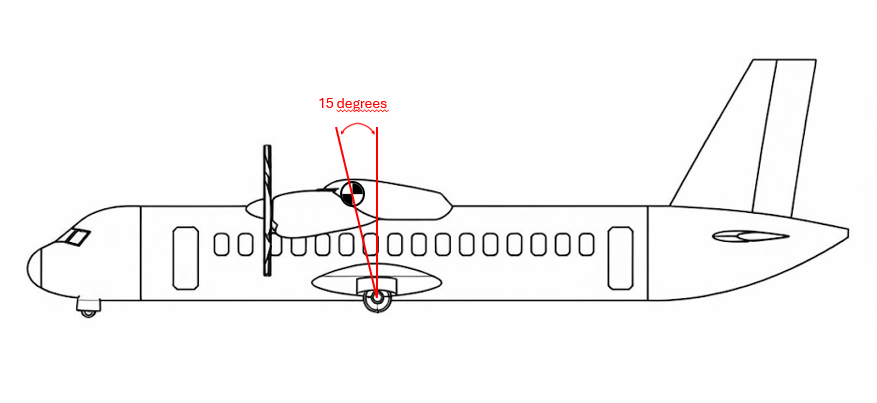
\includegraphics[width=\linewidth]{images/posicionamento longitudinal do trem de pouso.png}
        \caption{Posionamento longitudinal do trem de pouso.}
        \label{fig:longitudinal}
    \end{minipage}
\end{figure}


\subsubsection{Configuração final}

A configuração final foi confirme a imagem \ref{fig:configuração final do trem de pouso}.

\begin{figure}[H]
    \centering
    \begin{minipage}{0.8\textwidth} % Ajuste o 0.8 para aumentar ou diminuir o tamanho
        \centering
        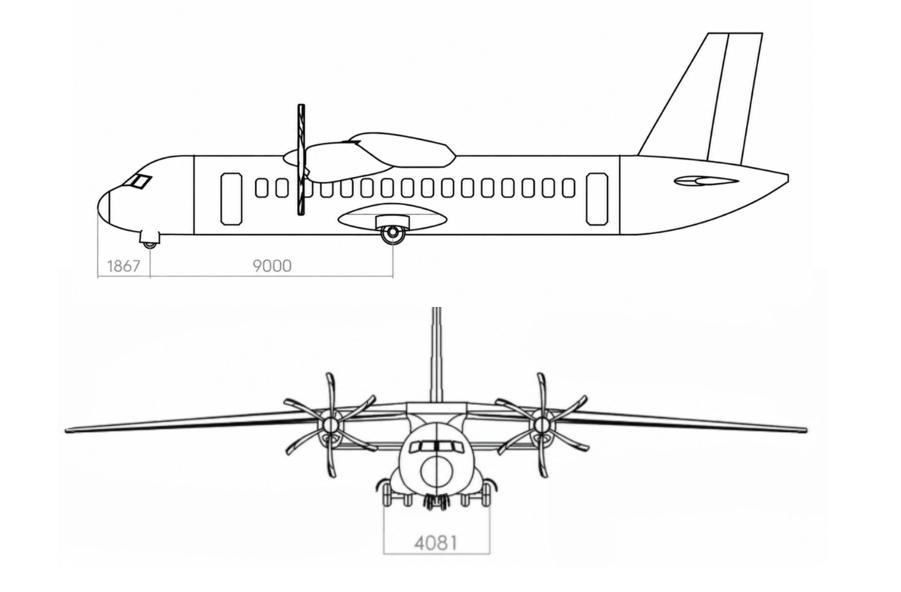
\includegraphics[width=\linewidth]{images/final trem de pouso.png}
        \caption{Configuração final do trem de pouso.}
        \label{fig:configuração final do trem de pouso}
    \end{minipage}
\end{figure}

\section{Dimensionamento de Sistemas}

\subsection{Sistema Hidráulico}

De acordo com o regulamento 14 CFR Part 25, Seção 25.1435, os componentes conectados ao sistema hidráulico principal devem ser projetados para suportar pressões de teste e de ruptura estabelecidas em função da Design Operating Pressure (DOP). Por meio de uma análise comparativa com aeronaves comerciais de porte semelhante, decidiu-se a utilização de uma DOP de 3000 psi, que representa uma prática comum da indústria para essa categoria de aeronaves. Dessa forma, esse valor foi adotado como pressão de operação de projeto para o dimensionamento preliminar do sistema hidráulico.\\
Além disso, a Design Operating Pressure (DOP) influencia diretamente o dimensionamento dos atuadores hidráulicos, uma vez que, para uma mesma força requerida, o aumento da pressão de operação permite a utilização de cilindros com menor área efetiva. Entretanto, pressões mais elevadas demandam componentes mais robustos, sofisticados e de maior custo, característica comum em aeronaves de transporte de passageiros de maior porte.\\
Para a elaboração do diagrama simplificado do sistema hidráulico, além do atendimento aos requisitos normativos, foi utilizado como referência o manual da aeronave ATR 72-600, por se tratar do modelo com características operacionais e de porte mais semelhantes à aeronave desenvolvida neste trabalho.\\
 A tabela abaixo foi estruturada com base na tabela original do regulamento, a qual encontra-se disponível na página 96, seção 25.1435, item a.
\begin{table}[H]
\centering
\caption{Fatores de pressão de ensaio e pressão última para componentes do sistema hidráulico.}
\label{tab:pressao_hidraulica}

\begin{tabular}{|p{8cm}|c|c|}
\hline
\textbf{Elemento} & \textbf{Ensaio (xDOP)} & \textbf{Última (xDOP)} \\
\hline
Tubulações e conexões & 4.500 psi & 9.000 psi\\
\hline
Vasos de pressão contendo gás (alta pressão, ex.: acumuladores) & 9.000 psi& 12.000 psi\\
\hline
Vasos de pressão contendo gás (baixa pressão, ex.: reservatórios) & 4.500 psi & 9.000 psi \\
\hline
Mangueiras & 6.000 psi & 12.000 psi \\
\hline
Demais componentes & 4.500 psi& 6.000 psi \\
\hline
\end{tabular}
\end{table}
 Adicionalmente, o requisito exige que os integrantes do sistema sejam capazes de suportar a pressão operacional de projeto juntamente com as cargas estruturais máximas previstas sem deformação que prejudique sua função, isto inclui suportar as cargas aerodinâmicas, as cargas devido a pressão interna, a vibrações, entre outras. Ademais, a tripulação deve ser informada imediatamente em caso de algum tipo de falha e possui meios para monitorar e ser alertada em caso de algum problema do sistema.\\
 Em resumo, o regulamento exige que:
 \begin{itemize}
     \item Cada componente suporte as pressões indicadas na Tabela \ref{tab:pressao_hidraulica};
     \item O sistema suporte cargas estruturais e vibrações;
     \item Não ocorram rupturas mesmo em condições extremas;
     \item Deve haver proteção contra ciclos de fadiga;
     \item Monitoramento pela tripulação;
     \item Vazamentos perigosos sejam minimizados;
     \item O sistema seja validado por testes de desempenho, fadiga e operação em voo.
 \end{itemize}
\vspace{0.5 cm}

 Para cumprir as exigências precisamos assegurar que alguns critérios sejam satisfeitos:
 \begin{itemize}
     \item As informações do sistema hidráulico precisam ser exibidas no cockpit;
     \item Deve haver alguma redundância para minimizar as chances de falha;
     \item Deve haver alertas sonoros para falhas e alerta emitidos para indicar que o sistema está apto, exemplo: PTU do A320.
     \item Em caso de falha nem todo sistema poderá ser comprometido;
     \item As bombas hidráulicas precisam ter acionamento via fonte AC e, quando disponível, fonte DC, para o caso em que as baterias estiverem suprindo a demanda.
 \end{itemize}

 Dessa forma, além dos critérios acima estabelecidos e levando em consideração o estudo do sistema hidráulico do ATR 72-600 um diagrama simplificado do sistema foi elaborado conforme abaixo:

A imagem acima apresenta uma versão simplificada da arquitetura do sistema hidráulico proposto, destacando seus principais componentes. De maneira semelhante à aeronave de referência, o sistema é composto por dois circuitos hidráulicos independentes, responsáveis pelo fornecimento do fluxo hidráulico aos consumidores da aeronave.\\
Ambos os circuitos são interligados por uma válvula de controle acionada por meio de um \textit{\textbf{push button}}, permitindo a transferência de fluido entre os sistemas em caso de falha de um dos retornos. Dessa forma, garante-se a continuidade do fornecimento hidráulico aos equipamentos essenciais da aeronave.\\
Adicionalmente, cada sistema possui seu próprio acumulador hidráulico e um conjunto independente de alimentação elétrica para as bombas hidráulicas. O sistema azul é alimentado pelo barramento elétrico BUS 1, enquanto o sistema verde é alimentado pelo BUS 2. Essa segregação aumenta a confiabilidade do projeto, uma vez que uma eventual falha elétrica em um dos barramentos não compromete completamente a capacidade de geração e distribuição de potência hidráulica da aeronave.\\
O reservatório hidráulico possui níveis de monitoramento destinados à detecção precoce de falhas e à garantia da operação segura do sistema. Um alerta de baixa quantidade de fluido deve ser acionado quando o nível atingir o valor indicado pela terceira linha preta pontilhada. Esse alerta tem caráter preventivo e visa informar a tripulação sobre a necessidade de inspeção ou manutenção do sistema.\\
Além disso, um alerta de emergência deve ser apresentado no cockpit caso o nível de fluido atinja a linha vermelha, correspondente ao limite mínimo admissível definido em projeto. Nessa condição, a quantidade de fluido disponível pode não ser suficiente para atender às demandas hidráulicas críticas da aeronave, comprometendo a confiabilidade e a disponibilidade do sistema. \\
Para calcular a  mínima de capacidade de fluído que deve estar disponível em tanque, um procedimento simplificado foi adotado, considerando a equação de momento em torno das articulações das superfícies de comando (Equação \ref{eq:moment-articu}), margem de segurança e sistema de frenagem.
\begin{equation}
    H = \frac{1}{2} \cdot \rho \cdot V \cdot S_c \cdot \bar{\bar{c_c}} \cdot C_H
    \label{eq:moment-articu}
\end{equation}
Em que:
\begin{itemize}
    \item V é a velocidade crítica das condições analisadas, sendo essas a VA e VD ;
    \item $S_c$ é a área da superfície;
    \item $\bar{\bar{c_c}}$ é  acorda média aerodinâmica da superfície analisada;
    \item $C_H$ é o coeficiente de momento em torno da articulação.
\end{itemize}

O coeficiente de momento por sua vez, pode ser descrito pela linearização abaixo, disponível nas notas de aulas de Estabilidade e Controle Ricardo U. Pinto (2012):
\begin{equation}
    C_H= b_0 + b_1 \cdot \alpha +b_2 \cdot \eta + b_3 \cdot \delta
\end{equation}
Considerou-se que as superfícies possuem perfis simétricos e com isso $b_0$ torna-se nulo, adicionalmente, descartou-se o uso de compensador e dessa forma a parcela de $b_3$ torna-se nula, asssim:
\begin{equation*}
    C_H = b_1 \cdot \alpha + b_2 \cdot \eta
\end{equation*}
As constantes $b_1$ e $b_2$ foram estimadas com base na aproximação proposta por ROSKAM, Jan. Airplane Design, Part VI em que:

\begin{equation}
\begin{aligned}
    b_1 &= C_{h_\alpha} \cdot D \\[6pt]
    b_2 &= C_{h_\delta} \cdot D
\end{aligned}
\end{equation}
Em que $C_{h_\alpha}$ e $C_{h_\delta}$ são estimados conforme as Figuras 10.63b e 10.69b do capítulo 10 de ROSKAM, Jan. Airplane Design, Part VI, respectivamente. Adicionalmente, o fator de correção 3D (D) é estimado por:
\begin{equation}
    D = \frac{C_{L_\alpha}}{C_{l_\alpha}}
\end{equation}

No qual o valor de $C_{L_\alpha}$ foi considerado como sendo o do avião sem flap e que foi obtido já com as correções para análise tridimensional da aeronave, $C_{l_\alpha}$ é aproximado por $2 \cdot \pi $ [$rad^{-1}$].\\
Assim obteve se um $C_H$ para cada superfície de controle principal e com isso o momento de cada superfície de controle principal (leme, aileron e profundor). Posteriormente, utilizou-se da pressão padrão de operação definida (DOP) e da seguinte formulação para calcular o volume de fluído requerido por essas superfícies.

\begin{equation}
    Volume = \frac{\frac{H}{braço}}{DOP } \cdot curso \cdot 1000
\end{equation}

De modo que o braço e curso foram baseados em método comparativo e pesquisa por valores padronizados na aviação, estimados em medições a partir do datum em catálogos de peças. \\
Assim, obtemos o volume para o acionamento das superfícies. Com relação ao freio e trem de pouso foi adotado o seguinte procedimento:

\begin{itemize}
    \item Para o trem de pouso, considerou-se para o cálculo que sua massa correspondia a 4,5\% do MTOW;
    \item  Um fator de arrasto e um curso de atuação foram estimados de modo que os resultados fossem compatíveis com os da aeronaves similares;
    \item Assim estimou-se a área e por fim o volume com base na DOP;
    \item Para os freios, considerou-se as quatro rodas e os quatro pistões por roda;
    \item Considerou-se um curso de 10 cm para os freios e uma área foi adotada para o pistão com base em um diâmetro de 85 mm, estimativa em escala;
    \item Obtendo assim o volume de fluído requerido pelos freios.
\end{itemize}

Dessa forma, foi realizada uma estimativa do consumo de fluido hidráulico considerando os atuadores das superfícies de comando sem a utilização de horn. Para a análise, foram consideradas apenas as condições correspondentes às velocidades de manobra ($V_A$) e de mergulho ($V_D)$). A partir dessas condições, foram obtidos os seguintes valores de capacidade  requerida para o reservatório hidráulico:

\begin{table}[H]
\centering
\caption{Dimensionamento do tanque hidráulico.}
\label{tab:dimensionamento_tanque}
\begin{tabular}{|c|c|c|}
\hline
\textbf{Velocidade} & \textbf{Demanda Simultânea Crítica} & \textbf{Volume com fator de tanque 1,2} \\
\hline
$V_A$ & 5.29 L & 6.96L \\
\hline
$V_D$ & 7,54 L & 9,63L \\
\hline
\end{tabular}
\end{table}


Portanto, considerando as hipóteses conservadoras adotadas no dimensionamento, obteve-se um reservatório hidráulico com capacidade máxima de 9,63 L. Adicionalmente, foi definido que o sistema deverá emitir um alerta de baixa quantidade de fluido quando o volume armazenado atingir 5,31 L.

Vale ressaltar que os valores obtidos mostram-se coerentes com aqueles encontrados em aeronaves da mesma categoria. Tendo em vista a referência adotada, o ATR 72-600 possui um reservatório hidráulico com capacidade máxima de aproximadamente 9,6 L, evidenciando que o dimensionamento realizado encontra-se dentro da faixa esperada para a aplicação considerada.



\begin{figure}[H]
    \centering
    \begin{minipage}{0.45\textwidth}
        \centering
        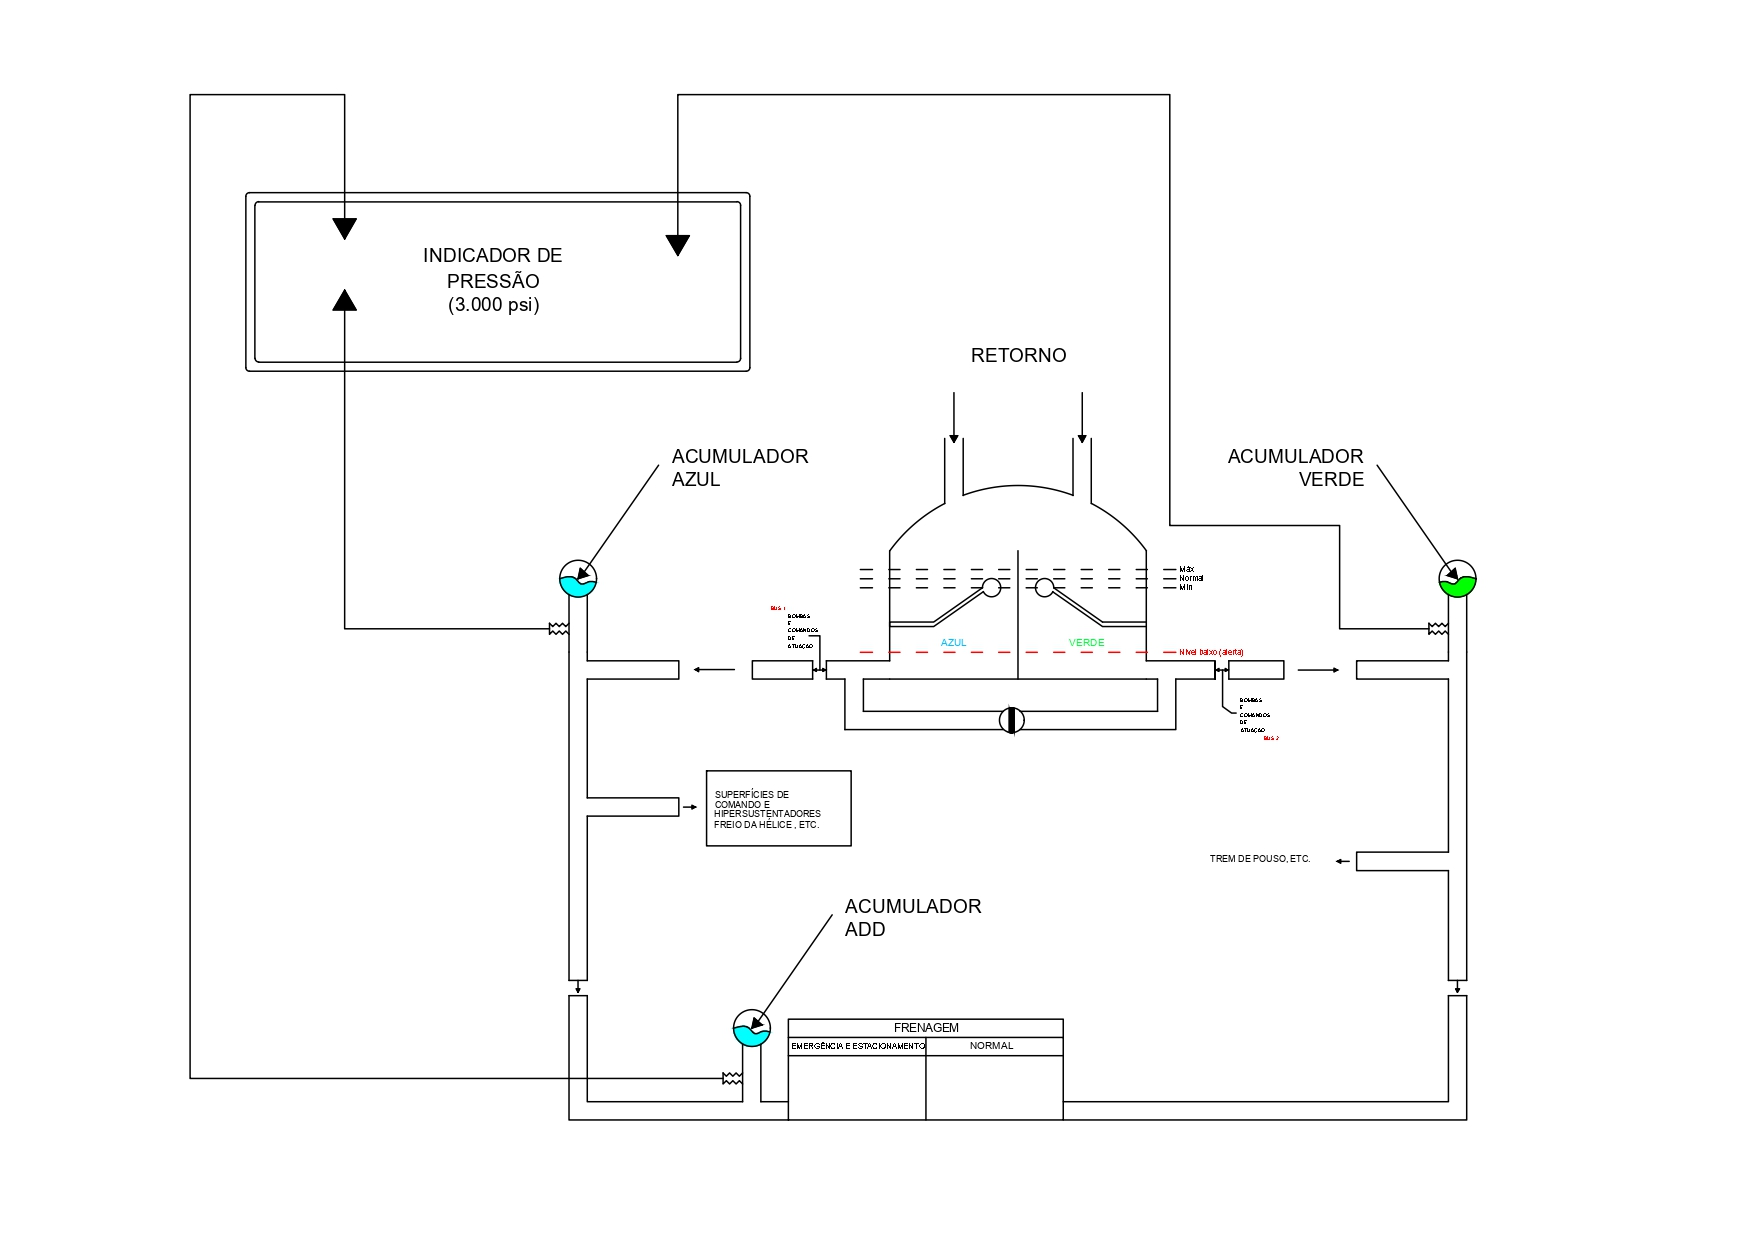
\includegraphics[width=\linewidth]{images/SistemaHidraulico.jpg}
        \caption{Diagrama simplificado do sistema hidráulico.}
        \label{sys_hidraulico}
    \end{minipage}
    \hfill
    \begin{minipage}{0.45\textwidth}
        \centering        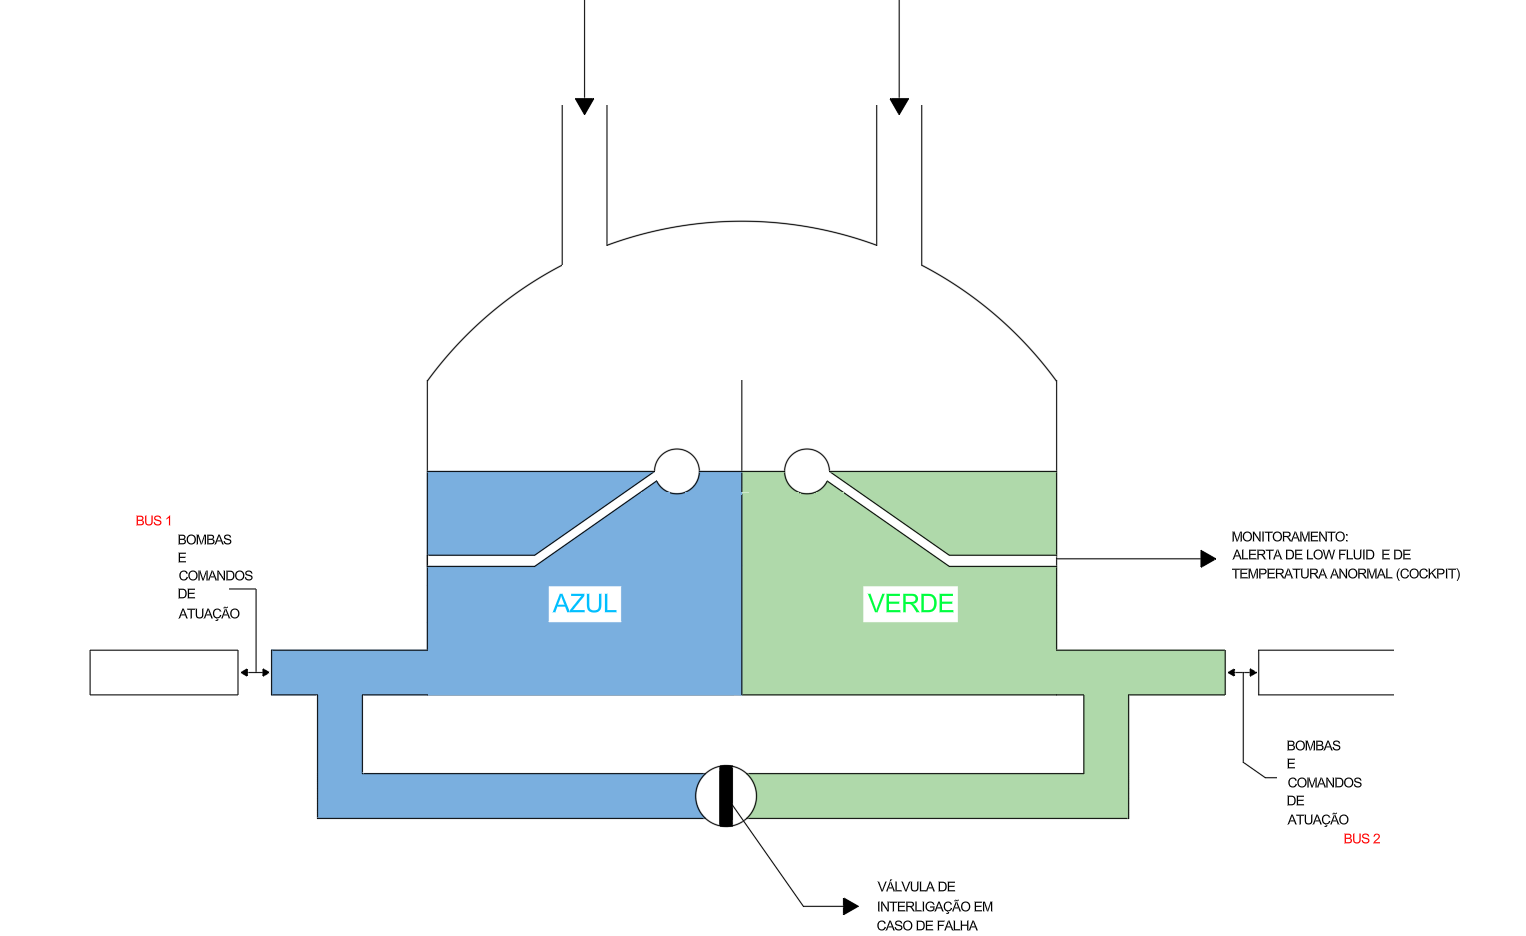
\includegraphics[width=\linewidth]{images/RESERVATÓRIO.png}
        \caption{Reservatório do fluido hidráulico}
        \label{Reservatorio_hidr}
    \end{minipage}
\end{figure}

\subsection{Environmental Control System}

O  ECS (\textit{Environmental Control System}) é responsável por garantir condições ambientais adequadas aos ocupantes da aeronave, proporcionando conforto e segurança. Suas principais funções incluem o fornecimento e a distribuição de ar para a cabine, o controle da temperatura, a remoção de contaminantes e a manutenção da pressão interna em níveis adequados. O dimensionamento preliminar foca apenas no sistema de pressurização da cabine e no sistema de ar-condicionado.

Conforme o requisito §25.841, aeronaves certificadas para operação até $25000 \ ft$, como este projeto, devem ter uma altitude máxima de cabine de $8000 \ ft$. Usando a atmosfera ISA, pode-se calcular o diferencial de pressão máximo no teto operacional.

\begin{equation}
    \Delta P=P_{cab}-P_{FL250}=10,92-5,45=5,47 \ psi
\end{equation} 

Deve haver uma válvula de alívio de pressão positiva para evitar a hiperpressurização. Considerando o valor típico de $\Delta P+0,5$, a válvula de ser dimensionada para $6,0 \ psi$. Para a válvula de alívio de pressão negativa (indispensável em situação de emergência de descida rápida), recomenda-se o dimensionamento para $-0,5 \ psi$. Posteriormente, o diferencial máximo da válvula de alívio será utilizado no cálculo de tensões circunferenciais e longitudinais na fuselagem. 

O balanço de massa deve ser feito para o dimensionamento preliminar dos PACK's - \textit{Pressurization Air Conditioning Kit}. Tem-se:
\begin{equation}
    \dot{m}_{supply}=\dot{m}_{outflow}+\dot{m}_{leakage}
\end{equation} onde $\dot{m}_{outflow}$ é a vazão da válvula de saída de ar, $\dot{m}_{supply}$ a vazão por PACK e $\dot{m}_{leakage}$ a taxa de vazamentos em juntas da fuselagem. Foram adotados dois PACK's (um por motor), permitindo redundância do sistema conforme o requisito §25.831.

Como critério de projeto, os vazamentos devem ser compensados. Logo, considerando o requisito §25.831 - a), a vazão fornecida $\dot{m}_{supply}$ deve ser:

\begin{align}
\dot{m}_{supply} &
= N_{PAX}\cdot 0,25\ \mathrm{kg/min}
+ \dot{m}_{leakage} \\
&= 74\cdot 0,25 + 2,5 \\
&= 21\ \mathrm{kg/min}
\end{align}

Já o balanço térmico considera a diferença entre a temperatura do ar sangrado do motor ($T_{bleed}$) e a da cabine de passageiros ($T_{cabin}$). Conforme a norma SAE AIR1168/3 \cite{SAE_AIR1168_3}, estima-se que o calor sensível por passageiro é de aproximadamente $75 \ W$. Considera-se $T_{bleed}=300 \ ^\circ C$  e $T_{cabin}=22 \ ^\circ C$ (valores típicos). Assim, calcula-se a carga térmica máxima por PACK:

\begin{align}
Q_{PACK} & =\dot{m}_{supply}\cdot c_p\cdot (T_{bleed}-T_{cabine})+75\cdot N_{pax} \\
&=  0,35\cdot 1,005 \cdot (200-22)+75 \cdot 74\\
&= 68,16 \ kW
\end{align}

A extração de ar do compressor do motor (\textit{bleed air}) representa uma penalização direta ao desempenho propulsivo da aeronave. Embora a carga térmica da cabine determine a demanda do sistema de condicionamento de ar, é a vazão de \textit{bleed} necessária para removê-la que define a potência efetivamente desviada do ciclo propulsivo. Assim, quanto maior a carga térmica, maior a vazão de ar requerida e, consequentemente, maior a redução da potência disponível no eixo e o aumento do consumo específico de combustível. Para mitigar esse impacto, busca-se minimizar a vazão extraída por meio da otimização do ECS e da redução das cargas térmicas da cabine. O valor de sangria máxima de 5\%. Por fim, nesta análise preliminar, não foram consideradas as cargas térmicas de aviônicos, equipamentos eletrônicos, sistemas embarcados e \textit{galley}.


\subsection{Sistema de Oxigênio}

O sistema de oxigênio da aeronave é composto por três componentes principais, os sistemas de armazenamento, de distribuição e de máscaras. Ainda é possível dividir as considerações a respeito do sistema de oxigênio entre cabine de comando, comissários de bordo e passageiros, visto que há diferentes requisitos, a exemplo da separação entre fonte de abastecimento para cabine de comando e cabine de passageiros ditada pela CS 25.1445.

O sistema de armazenamento de oxigênio dispõe de algumas opções: 
\begin{itemize}
    \item Oxigênio gasoso (ABO - \textit{Gaseous aviator breathing oxygen}): sistema que armazena o oxigênio como um gás, na forma de containers de alta ou baixa pressão, e apresenta como vantagem sua maior economia, mas tem como desvantagem seu peso e volume;
    \item Oxigênio líquido (LOX - \textit{Liquid aviator breathing oxygen}): sistema que armazena oxigênio em forma líquida e possui elevada taxa de expansão, com um litro de LOX sendo equivalente a 900 litros de ABO quando expandido. Porém, tem como desvantagem sua temperatura crítica de armazenamento (-127°C) e volatilidade quando em contato com derivados de petróleo;
    \item Geradores químicos de oxigênio: sistema se baseia na liberação de oxigênio por meio de reação química, geralmente usando clorato de sódio aquecido a cerca de 176°C. Apresenta como vantagem o menor peso e espaço ocupado quando comparado ao sistema ABO, mas tem como desvantagens a dificuldade em interromper a reação depois de iniciada e necessidade de precauções para evitar incêndios;
    \item \textit{Molecular sieve oxygen generators} (MSOG): sistema que separa o oxigênio dos demais gases presentes no ar ambiente, mas não é comumente utilizado na aviação civil \cite{OxiEquip}.
\end{itemize}

O sistema de distribuição apresenta como opções:
\begin{itemize}
    \item Sistemas de demanda: fornecem oxigênio apenas quando o usuário inspira pela máscara. Pode ser do tipo diluente-demanda ou pressão-demanda;
    \item Diluente-demanda: sistema capaz de misturar o ar da cabine e o oxigênio por meio de reguladores, podendo fornecer 100\% de oxigênio dependendo da altitude, e apresenta segurança no uso até 40.000 pés; 
    \item Pressão-demanda: sistema que aplica pressão positiva de oxigênio para promover o fluxo e pressurizar os pulmões do usuário, o que os torna seguros para uso acima de 40000 pés;
    \item Fluxo contínuo: sistema que fornece oxigênio durante todo o tempo que o usuário está com a máscara, coletando o oxigênio durante o tempo de exalação em um saco de reservatório. Geralmente, esse sistema é fornecido para passageiros \cite{SistemasANAC}.
\end{itemize}

Por fim, quanto às máscaras e cânulas, tem-se entre as opções:
\begin{itemize}
    \item Cânulas nasais: consistem em um tubo posicionado sob o nariz do usuário, que propiciam mais conforto do que as máscaras, mas podem não fornecer fluxo de oxigênio adequado. Atualmente, para operações acima de 18.000 pés, os regulamentos exigem que o sistema de oxigênio seja equipado com máscaras ao invés de cânulas \cite{SistemasANAC};
    \item Máscaras oronasais “\textit{re-breather}”: máscara acoplada a um saco de reservatório para coleta do ar exalado, o qual é misturado ao oxigênio do sistema. Essas máscaras são as mais comuns e baratas, e podem ser usadas com segurança até 25000 pés;
    \item Máscaras “\textit{quick-don}”: máscaras que podem ser colocadas com uma mão em até 5 segundos e possuem design que permite o uso de óculos. Podem ser utilizadas em altitudes de até 40000 pés;
    \item \textit{Airline drop-down units (Dixie cup)}: essas máscaras são similares à oronasal “re-breather”, mas possuem modificações que permitem seu uso até 40000 pés \cite{OxiEquip}.
\end{itemize}

Em razão da aeronave ser pressurizada, o uso de oxigênio dá-se em momentos de emergência e primeiros socorros, sendo crítico, por exemplo, caso ocorra uma despressurização da aeronave. Portanto, a escolha dos componentes do sistema se baseia nos requisitos aplicáveis a aeronaves pressurizadas com motores a turbina, que de maneira geral tratam do uso de oxigênio suplementar para descidas de emergência, e comparação com aeronaves similares. Assim, é considerado para o projeto o tempo de fornecimento de oxigênio, capacidade da aeronave, teto de serviço e requisitos para equipamentos.

Para os tripulantes de voo, definindo que será utilizado um sistema de demanda, que permite economia de oxigênio em 50\% a 85\%, é necessário um suprimento de 2 horas que garanta fluxo de 20 litros por minuto BTPS (\textit{Body Temperature and Pressure, Saturated}), conforme CS 25.1443. Além do cilindro de oxigênio capaz de satisfazer a necessidade citada, o regulamento informa que deve haver meios que permitam à tripulação usar oxigênio não diluído a seu critério, o que pode ser realizado por meio do seletor de oxigênio de diluição automática \cite{EASA25}. Ademais, como parte do equipamento para a tripulação da cabine de comando opta-se por máscaras do tipo “\textit{quick-don}”, em razão da sua característica de rápida colocação e compatibilidade com uso de óculos de correção.

Para a cabine de passageiros, a quantidade de suprimento de oxigênio deve ser suficiente para fornecer um mínimo de 10 minutos a todos os ocupantes. Ademais, assumindo que a aeronave é capaz de descer até o nível de 14000 pés dentro de 4 minutos em caso de despressurização, deve ser fornecido um suprimento de oxigênio a todos os ocupantes durante a descida e, considerando também o tempo até que a aeronave atinja 10000 pés, 30 minutos de oxigênio a pelo menos 10\% dos ocupantes \cite{EASA25}.

Desse modo, define-se que a aeronave possuirá suprimento capaz de fornecer um fluxo com 30 litros por minuto (BTPS) a todos os passageiros durante a descida e, pelo restante do tempo, um fluxo de 15 litros por minuto dimensionado para 30\% dos passageiros, a fim de atender aos requisitos da CS 25.1443 de maneira conservadora, mas também garantir que a aeronave não apresente excesso de peso quando operando em configuração cargueiro ou esteja superdimensionada para operações com transporte de passageiros abaixo da capacidade máxima. O oxigênio será fornecido aos passageiros por meio de um fluxo contínuo, a partir do uso de máscaras “\textit{re-breather}”, as quais possuem um saco de reservatório que coleta o oxigênio durante todo o tempo que o usuário a utiliza, sendo esta uma alternativa segura, barata e comum para a atitude de operação da aeronave.

Define-se também que serão disponibilizados cilindros de oxigênio portáteis aos tripulantes de cabine, a fim de permitir sua movimentação e atuação em eventuais primeiros socorros, além de estar em conformidade com o CS 25.1447 \cite{EASA25}. Considera-se que o fornecimento ocorrerá com o mesmo fluxo de litros por minutos descrito anteriormente, com cilindro de capacidade para 300 litros de oxigênio por membro da tripulação, conforme sugerido pelo regulamento.

Por fim, adota-se como sistema de armazenamento para cabine de passageiro os geradores químicos de oxigênio, devido ao seu menor peso, enquanto para cabine de comando será utilizado o ABO, em razão de ser mais econômico e por sua desvantagem de maior peso não ser tão significativa dada a menor demanda de volume dos cilindros.


\subsection{Auxiliary Power Unit (APU)}

A APU (\textit{Auxiliary Power Unit}) é uma pequena turbina a gás instalada na aeronave, normalmente na cauda, cuja função é gerar potência elétrica e pneumática independente dos motores principais. Em solo, ela permite alimentar os sistemas elétricos, o ar-condicionado da cabine e, em muitos casos, fornecer ar sangrado (\textit{bleed air}) para a partida dos motores, dispensando o uso de unidades externas de solo (\textit{Ground Power Unit} - GPU e \textit{Ground Air Unit} - GAU). Em voo, atua ainda como fonte redundante de energia em caso de falha dos geradores dos motores.

Para esta aeronave, no entanto, optou-se por não incorporar uma APU convencional ao projeto. O motor PW127M utiliza partida elétrica a partir da bateria da aeronave ou de uma fonte externa de energia (GPU elétrico), o que já elimina a principal justificativa pneumática para a existência de uma APU nesta classe de motorização.

 A solução adotada para suprir energia elétrica e pneumática em solo é a utilização de um dos motores com a hélice travada por um freio, acionando o gerador e o sistema pneumático normalmente. Essa configuração, chamada \textit{Hotel Mode} evita o peso, o custo de manutenção e o consumo de espaço na cauda associados a uma APU dedicada.

\subsection{Sistema de Proteção Contra Gelo e Degelo}
\label{subsec:degelo}

O sistema de proteção contra gelo e chuva é projetado para garantir a operação segura da aeronave em condições meteorológicas severas de congelamento em voo (\textit{icing conditions}), atendendo estritamente aos requisitos de certificação do RBAC 25 (§25.1419). Para uma aeronave comercial regional turboélice equipada com motores Pratt \& Whitney PW127M, a arquitetura de proteção adota um modelo híbrido fracionado em três níveis funcionais, combinando descongelamento pneumático e prevenção eletrotérmica.

A atuação do sistema de degelo pneumático promove a fratura e o desprendimento do gelo acumulado no bordo de ataque da asa e o desprendimento de placas de gelo das pás da hélice pela ação da força centrífuga e do aquecimento elétrico, restauram a geometria original do perfil aerodinâmico, reestabelecendo as condições nominais de escoamento. 

\paragraph{Bordo de ataque das asas:} Foi selecionado o uso de botas infláveis de borracha para os bordos de ataque da asa, devido à necessidade de minimizar a extração de potência no eixo ($SHP$) e a sangria de ar dos compressores do motor. Diferente de sistemas contínuos de sangria por ar quente, comuns em jatos comerciais de grande porte, o sistema pneumático demanda apenas pequenos surtos de pressão de ar comprimido da linha de alta pressão (HP) para os distribuidores. Isso preserva a margem de tração de decolagem em pistas curtas e reduz a penalidade de consumo específico de combustível em cruzeiro.

As botas são confeccionadas em elastômero sintético (borracha preta vulcanizada). Em conformidade com as diretrizes de projeto e manutenção, a borracha permanece sem pintura decorativa ou revestimento colorido, prevenindo a degradação química do material e fraturas superficiais por exposição aos raios UV e reagentes.
Além disso, o sistema de botas na asa é compartimentado ao longo da envergadura em seções internas e externas por semienvergadura. A alimentação de ar comprimido é cruzada entre as saídas dos dois motores. Esse arranjo assegura que, em caso de falha mecânica ou perfuração em uma das botas, a seção remanescente garanta o controle de rolamento (\textit{roll control}) atuando sobre os ailerons.

\paragraph{Empenagem Horizontal e Hélices:}Para a empenagem horizontal e as hélices, adota-se o aquecimento por resistência elétrica (\textit{eletrotérmico}) onde:
Para a Empenagem Horizontal é empregado O uso de resistências elétricas no bordo de ataque, que evita a necessidade de estender tubulações de ar quente ao longo de toda a fuselagem até a cauda, simplificando a montagem estrutural, eliminando riscos de vazamento térmico e reduzindo a massa global do sistema fixo;
e para Hélices e Admissão, A raiz das pás da hélice Hamilton Standard 568F (6 pás) e as entradas de ar do motor é utilizado elementos eletrotérmicos integrados, garantindo a eliminação do gelo por aquecimento local combinado à ação da força centrífuga.
Além das duas regiões, as janelas do cockpit também possuem aquecedor elétrico para evitar má visibilidade dos pilotos.

\paragraph{Vantagens do Sistema:} O sistema apresenta como principais vantagens a alta eficiência energética, obtida pela redução substancial na extração de potência do ciclo térmico do motor em comparação com sistemas pneumáticos contínuos; a independência operacional em relação ao ECS, uma vez que a conexão é realizada a montante das válvulas dos \textit{packs} do sistema de ar condicionado, garantindo que o degelo permaneça funcional mesmo em cenários de corte manual ou falha dos \textit{packs}; e a massa reduzida, proporcionada pelo baixo peso estrutural do elastômero e das linhas flexíveis de alimentação.

\paragraph{Sistema de Detecção de Gelo:} A identificação precoce da formação de gelo é realizada por um detector óptico instalado na fuselagem dianteira, que monitora a variação da reflexão de luz e a perda de transparência na superfície do sensor. Ao identificar o congelamento, o dispositivo sinaliza o \textit{Flight Warning System} (FWS), permitindo o disparo automático ou o acionamento preventivo manual dos sistemas de degelo pneumático e eletrotérmico.

\paragraph{Limitações e Operação:} O sistema de degelo (\textit{de-icing}) é acionado na presença de acúmulo inicial de camada de gelo, para que o ciclo de inflação do elastômero promova a fratura e o desprendimento aerodinâmico do bloco. Este acionamento é controlado por um temporizador com dois ciclos: ciclo rápido (1 minuto) para acúmulo acentuado e ciclo lento (3 minutos), para temperaturas baixas ($OAT < -10^\circ\text{C}$).

\subsubsection{Dimensionamento, Estimativa de Massa e Integridade do CG}

A pressão operacional do distribuidor pneumático é regulada entre $15\text{ psi}$ e $23\text{ psi}$, com o ar extraído da linha HP a montante da válvula do ECS. A estimativa de massa total do sistema de proteção contra gelo (incluindo 4 botas de borracha, 2 válvulas solenoides, atuadores elétricos, 2 sensores ópticos de detecção de gelo e fiação) é consolidada na Tabela~\ref{tab:massa_degelo}.

\begin{table}[H]
\centering
\caption{Estimativa de massa e distribuição dos componentes do sistema de degelo.}
\label{tab:massa_degelo}
\resizebox{\textwidth}{!}{%
\begin{tabular}{|c|c|c|c|c|}
\hline
\textbf{Componente} & \textbf{Qtd.} & \textbf{Tipo de Proteção} & \textbf{Massa Total (kgf)} & \textbf{Estação $X$ (m)} \\ \hline
Botas da Asa (Interna/Externa) & 4 & Pneumática (Borracha) & 42,0 & $11,20$ \\
Botas da Empenagem Horizontal & 2 & Eletrotérmica / Pneumática & 18,0 & $24,80$ \\
Resistências das Hélices & 12 & Eletrotérmica & 15,0 & $8,10$ \\
Aquecimento de Para-brisas & 2 & Filamentos Elétricos & 12,0 & $2,80$ \\
Sondas, Pitots e Sensores & 13 & Eletrotérmica & 8,0 & $1,50$ \\
Válvulas, Distribuidores e Tubos & --- & Pneumática / Elétrica & 25,0 & $11,80$ \\ \hline
\textbf{Total do Sistema} & --- & --- & \textbf{120,0} & $\mathbf{12,35}$ \\ \hline
\end{tabular}
}
\end{table}

A massa total de $120,0\text{ kgf}$ do sistema é integrada ao grupo de \textit{Equipamentos Fixos e Sistemas} no cálculo do $OEW$ (Tabela 4.7 e Tabela 11.1). Como o braço médio de atuação do sistema posiciona-se na estação $X = 12,35\text{ m}$ (próximo à região do bordo de ataque da CMA da asa e da transição com a cauda), o impacto no balanço de momentos mantém o envelope do Centro de Gravidade ($CG$) dentro do intervalo operacional seguro ($17,9\%\,\bar{c}$ a $45,9\%\,\bar{c}$).

A Tabela~\ref{tab:posicoes_degelo} resume a distribuição espacial e a tecnologia adotada para cada superfície crítica da aeronave. Enquanto a Figura~\ref{fig:posicao_degelo} as apresenta graficamente.

\begin{table}[htbp]
\centering
\caption{Mapeamento de proteção contra gelo por componente da aeronave.}
\label{tab:posicoes_degelo}
\resizebox{\textwidth}{!}{%
\begin{tabular}{|c|c|c|}
\hline
\textbf{Componente} & \textbf{Tecnologia Adotada} & \textbf{Detalhamento e Posição} \\ \hline
Bordo de Ataque da Asa & Botas Pneumáticas & Elastômero preto em seções bipartidas ao longo da envergadura. \\
Empenagem Horizontal & Resistência Elétrica & Elementos eletrotérmicos no bordo de ataque do estabilizador. \\
Hélices & Resistência Elétrica & Filamentos na raiz das 6 pás de cada hélice (próximo ao \textit{spinner}). \\
Carenagem do Motor & Botas / Sangria HP & Proteção dos bordos de ataque da admissão de ar do PW127M. \\
Controles de Voo (\textit{Horns}) & Resistência Elétrica & Aquecimento nas pontas de compensação aerodinâmica de ailerons e leme. \\
Para-brisa Frontal & Vidro Eletrotérmico & Filamentos internos para aquecimento, desembaçamento e degelo. \\
Sondas de Voo & Aquecimento Direto & 3 tubos Pitot, 6 tomadas estáticas, 2 sensores TAT e 2 AOA. \\ \hline
\end{tabular}
}
\end{table}

\begin{figure}[H]
    \centering
    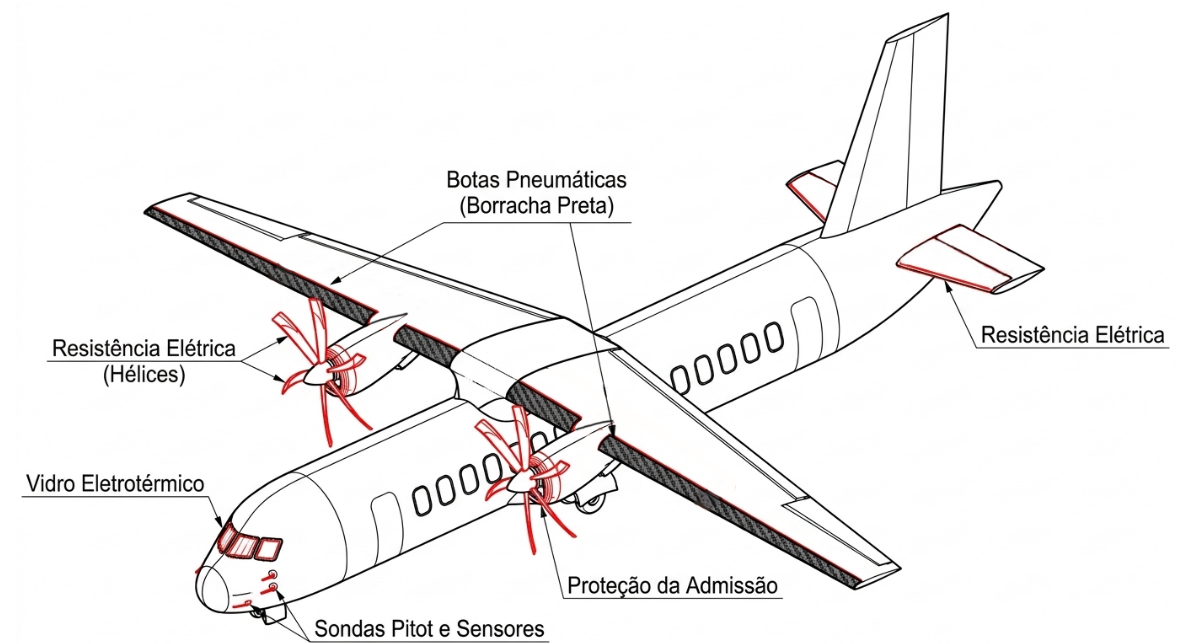
\includegraphics[width=1\textwidth]{images/Posicao sist degelo.png} 
    \caption{Posicionamento do sistema de Degelo na Aeronave}
    \label{fig:posicao_degelo}
\end{figure}